% Este archivo es parte de la memoria del proyecto fin de carrera
% de Manuel López Urbina. Protegida bajo la licencia GFDL.
% Para más información, la licencia completa viene incluida en el
% fichero fdl-1.3.tex

% Copyright (C) 2012 Manuel López Urbina

\chapter{Software de reconocimiento}
\label{chap:reconocimiento}

Una vez descritos los diferentes elementos hardware utilizados y la metodología de desarrollo empleada, en el presente capítulo  sucesivos se realizará un profundo análisis de las técnicas y problemas detectados durante el desarrollo, comenzando en el presente tema por el software de reconocimiento. Este subsistema ha sido elaborado siguiendo el modelo de construcción por prototipos.\\

A modo introductorio, destacar que el software de reconocimiento ha sido elaborado haciendo uso de la biblioteca OpenCV para el lenguaje C. Esta biblioteca incluye los elementos necesarios para el tratamiento de imágenes para, como se ha descrito en la sección \ref{sec:objetivos} de objetivos, proporcionar al vehículo de un sistema de reconocimiento de señales de tráfico.\\

Las señales de tráfico detectables por el sistema serán las siguientes:\\

\begin{figure}[H]
  \begin{center}
    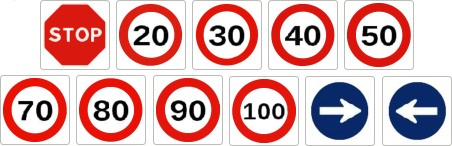
\includegraphics[scale=1]{seniales2.png}
  \end{center}
  \caption{Conjunto de señales de tráfico detectables por el sistema.}
  \label{conjunto-señales-rp}
\end{figure}

Entre las señales incluidas disponemos las diferentes señales indicadoras de velocidad máxima, existiendo desde la de 20 km/h hasta la de 100 km/h con el objetivo de poder ajustar automáticamente la velocidad del vehículo en función de la señal detectada.\\

Por otro lado existen las señales indicadoras de dirección obligatoria, con el fin de efectuar giros y la señal de stop con el propósito de efectuar paradas de manera automática.\\

Para la elaboración del sistema ha sido necesario el desarrollo de tres prototipos. En las sucesivas secciones del tema se describirán cada uno de los ellos junto con los problemas detectados y motivos por los que finalmente se acabaron desechando junto con las soluciones adoptadas.

\section {Primer prototipo}

Para el desarrollo del primer prototipo se han empleado las siguientes técnicas:

\begin{enumerate}
\item Segmentación por color de la imagen de entrada.
\item Eliminación de objetos pequeños resultantes con área inferior a un determinado valor.
\item Extracción de la imagen de objetos existentes.
\item Comparación de cada uno de los objetos con plantillas para su identificación.
\end{enumerate}

\subsection{Obtención de la imagen}

El paso previo de todo sistema de reconocimiento de objetos es la extracción de características a partir de unos datos de entrada para su posterior análisis. La información de entrada es proporcionada al sistema mediante una imagen, la cual es obtenida a través de la cámara que dota el vehículo.\\

Sin embargo, lo único que se recibe es una matriz de números desde la cámara.\\

\begin{figure}[H]
  \begin{center}
    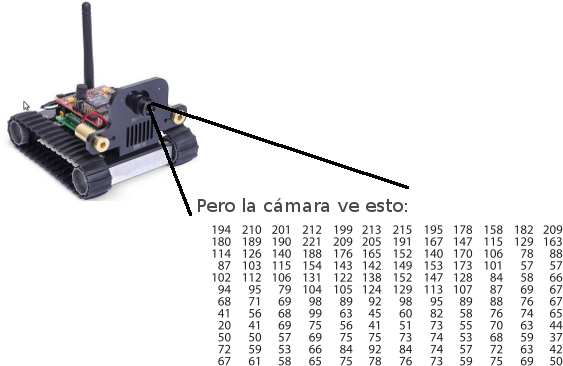
\includegraphics[scale=0.5]{datos-camara.png}
  \end{center}
  \caption{Interpretación de una imagen por parte de una cámara}
  \label{imagen-entrada-rp}
\end{figure}

Dicha matriz de números es recibida por el ordenador para su posterior interpretación y tratamiento\footnote{El procedimiento empleado para la transmisión de la imagen desde el vehículo al computador de manera física queda reflejado en el tema \ref{chap:dispositivos-hardware} correspondiente al montaje de los dispositivos hardware.}. \\

A continuación se muestra el código realizado en OpenCV para la obtención de las imágenes a partir de una cámara:\\

\underline{Algoritmo de obtención de imágenes}\\
\begin{Verbatim}[commandchars=\\\{\}]
\PY{c+cp}{#}\PY{c+cp}{include <stdio.h>}
\PY{c+cp}{#}\PY{c+cp}{include <stdlib.h>}
\PY{c+cp}{#}\PY{c+cp}{include "opencv}\PY{c+cp}{/}\PY{c+cp}{cv.h" }
\PY{c+cp}{#}\PY{c+cp}{include "opencv}\PY{c+cp}{/}\PY{c+cp}{highgui.h"}

\PY{k+kt}{int} \PY{n+nf}{main}\PY{p}{(}\PY{k+kt}{int} \PY{n}{argc}\PY{p}{,} \PY{k+kt}{char} \PY{o}{*}\PY{n}{argv}\PY{p}{[}\PY{p}{]}\PY{p}{)}
\PY{p}{\PYZob{}}
  \PY{n}{IplImage} \PY{o}{*}\PY{n}{img}\PY{o}{=}\PY{n+nb}{NULL}\PY{p}{;}

  \PY{k+kt}{char} \PY{n}{c}\PY{o}{=}\PY{n+nb}{NULL}\PY{p}{;}

  \PY{c+c1}{// Crea una ventana llamada Imagen}
  \PY{c+c1}{// con tamaño predeterminado.}
  \PY{n}{cvNamedWindow}\PY{p}{(}\PY{l+s}{"}\PY{l+s}{Imagen}\PY{l+s}{"}\PY{p}{,}\PY{n}{CV\PYZus{}WINDOW\PYZus{}AUTOSIZE}\PY{p}{)}\PY{p}{;}
 
  \PY{c+c1}{// Crea la conexion con la Webcam.}
  \PY{n}{CvCapture}\PY{o}{*} \PY{n}{captura} \PY{o}{=} \PY{n}{cvCaptureFromCAM}\PY{p}{(}\PY{o}{-}\PY{l+m+mi}{1}\PY{p}{)}\PY{p}{;}
 
   \PY{c+c1}{// Si la tecla pulsada es ESC se sale del bucle.}
   \PY{k}{while}\PY{p}{(}\PY{n}{c} \PY{o}{!}\PY{o}{=} \PY{l+m+mi}{27}\PY{p}{)} \PY{p}{\PYZob{}} 

    \PY{c+c1}{// Añade el frame capturado dentro de la imagen img.}
    \PY{n}{img} \PY{o}{=} \PY{n}{cvQueryFrame}\PY{p}{(}\PY{n}{captura}\PY{p}{)}\PY{p}{;}

    \PY{c+c1}{// PROCESAMIENTO DE LA IMAGEN.}
  
    \PY{c+c1}{// Se espera la pulsación de alguna tecla }
    \PY{c+c1}{// durante 10 milésimas de segundo.}
    \PY{c+c1}{// De ser alguna tecla pulsada, }
    \PY{c+c1}{// se almacena en la variable c.}
    \PY{n}{c} \PY{o}{=} \PY{n}{cvWaitKey}\PY{p}{(}\PY{l+m+mi}{10}\PY{p}{)}\PY{p}{;}
  \PY{p}{\PYZcb{}}

  \PY{c+c1}{// Liberación de la cámara.}
  \PY{n}{cvReleaseCapture}\PY{p}{(}\PY{o}{&}\PY{n}{captura}\PY{p}{)}\PY{p}{;}

  \PY{c+c1}{// Eliminamos todas las estructuras ventana existentes. }
  \PY{n}{cvDestroyAllWindows}\PY{p}{(}\PY{p}{)}\PY{p}{;} 
   
  \PY{k}{return} \PY{l+m+mi}{0}\PY{p}{;}
\PY{p}{\PYZcb{}}
\end{Verbatim}


Una vez obtenida la imagen, ésta es almacenada en la variable, \emph{img} del código anterior. A partir de ese instante se dispone de la base para aplicar la extracción de características y el procesamiento de la imagen que se desee aplicar añadiendo el código necesario en la parte interna del bucle del código mostrado. Una vez finalizado el procesamiento aplicado a la imagen capturada se obtiene un nuevo frame para continuar con el procesamiento de una nueva imagen mientras la tecla ESC no sea presionada.\\

Un ejemplo de una imagen de entrada capturada por la cámara y visionada en la pantalla del ordenador utilizando el código anteriormente mostrado puede ser el siguiente:\\

\begin{figure}[H]
  \begin{center}
    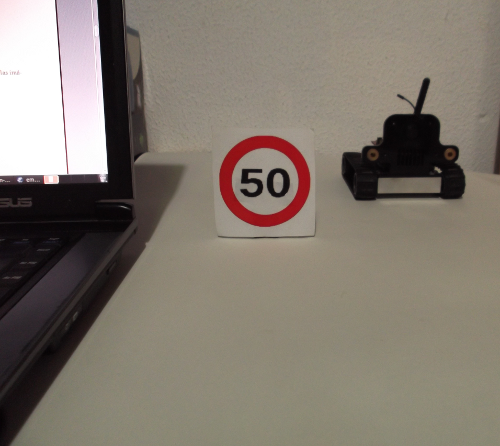
\includegraphics[scale=0.6]{im-entrada3.png}
  \end{center}
  \caption{Posible imagen de entrada al sistema.}
  \label{imagen-entrada-rp}
\end{figure}


\subsection{Extracción de características}
\label{sec:extraccion-caracteristicas}

Puesto que el fin es la detección de un objeto, la segmentación de la imagen es empleada para aislar en ella a todos los conjuntos de píxeles candidatos a ser el objeto a seguir o detectar. Como hemos visto en la imagen \ref{imagen-entrada-rp} las señales a detectar presentan colores llamativos, visualizándose en su contorno más externo los colores rojos y azules, siendo éstos los más representativos y predominantes. Por tanto resulta de especial utilidad la aplicación de una segmentación por color. Existen numerosos modelos de color utilizables para su realización como se ha descrito en la sección de \ref{def:modelos-color}.\\

Para la primera etapa del desarrollo del primer prototipo se ha empleado una técnica de segmentación por color siguiendo el modelo RGB. La finalidad de la segmentación es la de realizar una correcta selección de aquellos píxeles que según una determinada tonalidad resultan útiles para el posterior procesamiento e identificación de objetos. 

\subsubsection {Segmentación por color siguiendo el modelo RGB}
\label{sec:seg-color-rgb}

Dado que los colores predominantes de las señales a detectadas son los rojos y azules intensos se ha optado por la selección de ambas tonalidades, centrándonos, para este primer prototipo, en el color rojo exclusivamente.\\

Una vez decidido el color a identificar, resulta necesario conocer las tonalidades exactas y cómo ésta es representada por el ordenador. La solución fue crear una herramienta con la que al pinchar sobre una imagen, obtuviera de forma automática el color sobre el que se ha pulsado mostrando por pantalla el código del color en los tres canales: rojo, verde y azul. El programa se escribió en lenguaje C haciendo uso de la biblioteca OpenCV.\\

 En la figura \ref{fig:color-pixel} se puede observar el funcionamiento del programa mostrando el color sobre el que se ha hecho click, apreciándose como el último color seleccionado posee los valores 84, 70 y 202. Destacar que OpenCV invierte el orden de las componente empleando BGR en lugar de RGB. Es decir, azul, verde y rojo, presentando, por tanto, un valor numérico mayor en la tercera componente. Esto se debe a que el píxel pulsado en la imagen se corresponde con el contorno exterior de la señal de 50 km/h cuya tonalidad es roja y que predomina sobre las otras dos.\\

\begin{figure}[H]
  \begin{center}
    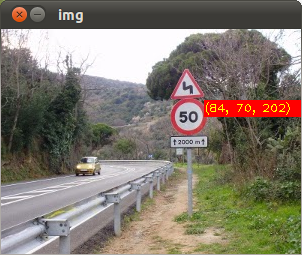
\includegraphics[scale=0.7]{color-pixel.png}
  \end{center}
  \caption{Programa elaborado para la obtención de los valores del píxel pulsado.}
  \label{fig:color-pixel}
\end{figure}

El código del programa elaborado se muestra a continuación:\\

\underline{Programa elaborado para la obtención del valor de un píxel en una imagen}\\
\begin{Verbatim}[commandchars=\\\{\}]
\PY{c+cp}{#}\PY{c+cp}{include "cv.h"}
\PY{c+cp}{#}\PY{c+cp}{include "highgui.h"}
\PY{c+cp}{#}\PY{c+cp}{include <stdio.h>}
\PY{c+cp}{#}\PY{c+cp}{include <stdlib.h>}

\PY{k+kt}{void} \PY{n+nf}{mouseHandler}\PY{p}{(}\PY{k+kt}{int} \PY{n}{event}\PY{p}{,} \PY{k+kt}{int} \PY{n}{x}\PY{p}{,} \PY{k+kt}{int} \PY{n}{y}\PY{p}{,} \PY{k+kt}{int} \PY{n}{flags}\PY{p}{,} \PY{k+kt}{void}\PY{o}{*} \PY{n}{param}\PY{p}{)}
\PY{p}{\PYZob{}}
    \PY{c+c1}{// Declaración de variables.}
    \PY{n}{IplImage}\PY{o}{*} \PY{n}{img0}\PY{p}{,} \PY{o}{*} \PY{n}{img1}\PY{p}{;}
    \PY{n}{CvFont}    \PY{n}{font}\PY{p}{;}
    \PY{n}{uchar}\PY{o}{*}    \PY{n}{ptr}\PY{p}{;}
    \PY{k+kt}{char}      \PY{n}{label}\PY{p}{[}\PY{l+m+mi}{20}\PY{p}{]}\PY{p}{;}

    \PY{n}{img0} \PY{o}{=} \PY{p}{(}\PY{n}{IplImage}\PY{o}{*}\PY{p}{)} \PY{n}{param}\PY{p}{;}
    \PY{n}{img1} \PY{o}{=} \PY{n}{cvCloneImage}\PY{p}{(}\PY{n}{img0}\PY{p}{)}\PY{p}{;}


    \PY{n}{cvInitFont}\PY{p}{(}\PY{o}{&}\PY{n}{font}\PY{p}{,} \PY{n}{CV\PYZus{}FONT\PYZus{}HERSHEY\PYZus{}PLAIN}\PY{p}{,} \PY{l+m+mf}{.8}\PY{p}{,} \PY{l+m+mf}{.8}\PY{p}{,} \PY{l+m+mi}{0}\PY{p}{,} \PY{l+m+mi}{1}\PY{p}{,} \PY{l+m+mi}{8}\PY{p}{)}\PY{p}{;}

    \PY{k}{if} \PY{p}{(}\PY{n}{event} \PY{o}{=}\PY{o}{=} \PY{n}{CV\PYZus{}EVENT\PYZus{}LBUTTONDOWN}\PY{p}{)}
    \PY{p}{\PYZob{}}
        \PY{c+c1}{// Se realiza la lectura del píxel pulsado.}
        \PY{n}{ptr} \PY{o}{=} \PY{n}{cvPtr2D}\PY{p}{(}\PY{n}{img1}\PY{p}{,} \PY{n}{y}\PY{p}{,} \PY{n}{x}\PY{p}{,} \PY{n+nb}{NULL}\PY{p}{)}\PY{p}{;}

        \PY{c+c1}{// Se muestra el valor RGB.}
        \PY{n}{sprintf}\PY{p}{(}\PY{n}{label}\PY{p}{,} \PY{l+s}{"}\PY{l+s}{(%d, %d, %d)}\PY{l+s}{"}\PY{p}{,} \PY{n}{ptr}\PY{p}{[}\PY{l+m+mi}{0}\PY{p}{]}\PY{p}{,} \PY{n}{ptr}\PY{p}{[}\PY{l+m+mi}{1}\PY{p}{]}\PY{p}{,} \PY{n}{ptr}\PY{p}{[}\PY{l+m+mi}{2}\PY{p}{]}\PY{p}{)}\PY{p}{;}
        
        \PY{c+c1}{// Se crea un rectángulo de color en la imagen...}
        \PY{n}{cvRectangle}\PY{p}{(} 
            \PY{n}{img1}\PY{p}{,}
            \PY{n}{cvPoint}\PY{p}{(}\PY{n}{x}\PY{p}{,} \PY{n}{y} \PY{o}{-} \PY{l+m+mi}{12}\PY{p}{)}\PY{p}{,}
            \PY{n}{cvPoint}\PY{p}{(}\PY{n}{x} \PY{o}{+} \PY{l+m+mi}{100}\PY{p}{,} \PY{n}{y} \PY{o}{+} \PY{l+m+mi}{4}\PY{p}{)}\PY{p}{,}
            \PY{n}{CV\PYZus{}RGB}\PY{p}{(}\PY{l+m+mi}{255}\PY{p}{,} \PY{l+m+mi}{0}\PY{p}{,} \PY{l+m+mi}{0}\PY{p}{)}\PY{p}{,}
            \PY{n}{CV\PYZus{}FILLED}\PY{p}{,}
            \PY{l+m+mi}{8}\PY{p}{,} \PY{l+m+mi}{0}
        \PY{p}{)}\PY{p}{;}
        \PY{c+c1}{// Y se dibuja los valores numéricos en su interior.}
        \PY{n}{cvPutText}\PY{p}{(}
            \PY{n}{img1}\PY{p}{,}
            \PY{n}{label}\PY{p}{,}
            \PY{n}{cvPoint}\PY{p}{(}\PY{n}{x}\PY{p}{,} \PY{n}{y}\PY{p}{)}\PY{p}{,}
            \PY{o}{&}\PY{n}{font}\PY{p}{,}
            \PY{n}{CV\PYZus{}RGB}\PY{p}{(}\PY{l+m+mi}{255}\PY{p}{,} \PY{l+m+mi}{255}\PY{p}{,} \PY{l+m+mi}{0}\PY{p}{)}
        \PY{p}{)}\PY{p}{;}

        \PY{c+c1}{// Finalmente se muestra la imagen.}
        \PY{n}{cvShowImage}\PY{p}{(}\PY{l+s}{"}\PY{l+s}{img}\PY{l+s}{"}\PY{p}{,} \PY{n}{img1}\PY{p}{)}\PY{p}{;}
    \PY{p}{\PYZcb{}}
\PY{p}{\PYZcb{}}


\PY{k+kt}{int} \PY{n}{main}\PY{p}{(}\PY{k+kt}{int} \PY{n}{argc}\PY{p}{,} \PY{k+kt}{char} \PY{o}{*}\PY{n}{argv}\PY{p}{[}\PY{p}{]}\PY{p}{)}\PY{p}{\PYZob{}}

    \PY{n}{IplImage}\PY{o}{*} \PY{n}{img}\PY{p}{,}\PY{o}{*}\PY{n}{hsv\PYZus{}image}\PY{p}{;}

    \PY{c+c1}{// Se comprueba que se ha introducido un argumento.}
    \PY{k}{if} \PY{p}{(}\PY{n}{argc} \PY{o}{!}\PY{o}{=} \PY{l+m+mi}{2}\PY{p}{)} \PY{p}{\PYZob{}}
        \PY{n}{printf}\PY{p}{(}\PY{l+s}{"}\PY{l+s}{Usage: %s <image>}\PY{l+s+se}{\PYZbs{}n}\PY{l+s}{"}\PY{p}{,} \PY{n}{argv}\PY{p}{[}\PY{l+m+mi}{0}\PY{p}{]}\PY{p}{)}\PY{p}{;}
        \PY{k}{return} \PY{l+m+mi}{1}\PY{p}{;}
    \PY{p}{\PYZcb{}}

    \PY{c+c1}{// Se realiza la carga de la imagen a partir de la ruta pasada }
    \PY{c+c1}{// como argumento de entrada.}
    \PY{n}{img} \PY{o}{=} \PY{n}{cvLoadImage}\PY{p}{(}\PY{n}{argv}\PY{p}{[}\PY{l+m+mi}{1}\PY{p}{]}\PY{p}{,} \PY{l+m+mi}{1}\PY{p}{)}\PY{p}{;}

    \PY{c+c1}{//Copia de la imagen de entrada en una nueva imagen.}
    \PY{n}{hsv\PYZus{}image} \PY{o}{=} \PY{n}{cvCloneImage}\PY{p}{(}\PY{n}{img}\PY{p}{)}\PY{p}{;} 
    
    \PY{c+c1}{//Transformacion a HSV}
    \PY{n}{cvCvtColor}\PY{p}{(}\PY{n}{img}\PY{p}{,} \PY{n}{hsv\PYZus{}image}\PY{p}{,} \PY{n}{CV\PYZus{}BGR2HSV}\PY{p}{)}\PY{p}{;}

    \PY{c+c1}{// Se crea una ventana con los eventos del ratón.}
    \PY{n}{cvNamedWindow}\PY{p}{(}\PY{l+s}{"}\PY{l+s}{img}\PY{l+s}{"}\PY{p}{,} \PY{l+m+mi}{1}\PY{p}{)}\PY{p}{;}
    \PY{n}{cvSetMouseCallback}\PY{p}{(}\PY{l+s}{"}\PY{l+s}{img}\PY{l+s}{"}\PY{p}{,} \PY{n}{mouseHandler}\PY{p}{,} \PY{p}{(}\PY{k+kt}{void}\PY{o}{*}\PY{p}{)}\PY{n}{hsv\PYZus{}image}\PY{p}{)}\PY{p}{;}

    \PY{n}{cvShowImage}\PY{p}{(}\PY{l+s}{"}\PY{l+s}{img}\PY{l+s}{"}\PY{p}{,} \PY{n}{hsv\PYZus{}image}\PY{p}{)}\PY{p}{;}
    \PY{n}{cvWaitKey}\PY{p}{(}\PY{l+m+mi}{0}\PY{p}{)}\PY{p}{;}

    \PY{c+c1}{// Eliminación de estructuras.}
    \PY{n}{cvDestroyAllWindows}\PY{p}{(}\PY{p}{)}\PY{p}{;}
    \PY{n}{cvReleaseImage}\PY{p}{(}\PY{o}{&}\PY{n}{img}\PY{p}{)}\PY{p}{;}
    \PY{n}{cvReleaseImage}\PY{p}{(}\PY{o}{&}\PY{n}{hsv\PYZus{}image}\PY{p}{)}\PY{p}{;}

    \PY{k}{return} \PY{l+m+mi}{0}\PY{p}{;}
\PY{p}{\PYZcb{}}
\end{Verbatim}


Una vez conocidos los umbrales sobre los que trabajar, siempre en torno a un pequeño margen, se procede a una criba de píxeles que entran dentro del citado rango.\\

El código mostrado a continuación recibe una imagen de entrada realizando su recorrido y activando en una nueva imagen binaria, originalmente inicializada a cero, con el valor 1 aquellos píxeles situados dentro del umbral de color indicado. El recorrido de la imagen se ha realizado utilizando la aritmética de punteros en lugar de las funciones consultoras propias de OpenCV con el fin de ganar en eficiencia.\\

\underline{Segmentación de una imagen siguiendo el modelo de color RGB}\\
\begin{Verbatim}[commandchars=\\\{\}]
\PY{n}{IplImage}\PY{o}{*} \PY{n}{segmentacion\PYZus{}RGB}\PY{p}{(}\PY{n}{IplImage}\PY{o}{*} \PY{n}{img}\PY{p}{)}\PY{p}{\PYZob{}}

  \PY{c+c1}{// Declaración de variables.}
  \PY{k+kt}{int} \PY{n}{altura}\PY{p}{,}\PY{n}{anchura}\PY{p}{,}\PY{n}{anchura\PYZus{}fila}\PY{p}{,}\PY{n}{canales}\PY{p}{;}
  \PY{n}{uchar} \PY{o}{*}\PY{n}{data}\PY{p}{;}
  \PY{k+kt}{int} \PY{n}{i}\PY{p}{,}\PY{n}{j}\PY{p}{;}
  
  \PY{c+c1}{// Recopilación de los datos de la imagen de entrada.}
  \PY{n}{altura} \PY{o}{=} \PY{n}{img}\PY{o}{-}\PY{o}{>}\PY{n}{height}\PY{p}{;}
  \PY{n}{anchura} \PY{o}{=} \PY{n}{img}\PY{o}{-}\PY{o}{>}\PY{n}{width}\PY{p}{;}
  \PY{n}{anchura\PYZus{}fila} \PY{o}{=} \PY{n}{img}\PY{o}{-}\PY{o}{>}\PY{n}{widthStep}\PY{p}{;}
  \PY{n}{canales} \PY{o}{=} \PY{n}{img}\PY{o}{-}\PY{o}{>}\PY{n}{nChannels}\PY{p}{;}
  \PY{n}{data} \PY{o}{=} \PY{p}{(}\PY{n}{uchar} \PY{o}{*}\PY{p}{)}\PY{n}{img}\PY{o}{-}\PY{o}{>}\PY{n}{imageData}\PY{p}{;}
     
  \PY{c+c1}{// Declaración e inicialización a cero de la imagen de salida.}
  \PY{n}{IplImage}\PY{o}{*} \PY{n}{img\PYZus{}selec\PYZus{}color}\PY{p}{;}  
  \PY{n}{img\PYZus{}selec\PYZus{}color} \PY{o}{=} \PY{n}{cvCreateImage}\PY{p}{(}\PY{n}{cvGetSize}\PY{p}{(}\PY{n}{img}\PY{p}{)}\PY{p}{,} \PY{n}{IPL\PYZus{}DEPTH\PYZus{}8U}\PY{p}{,}\PY{l+m+mi}{1}\PY{p}{)}\PY{p}{;}
  \PY{n}{cvZero}\PY{p}{(}\PY{n}{img\PYZus{}selec\PYZus{}color}\PY{p}{)}\PY{p}{;}

  \PY{c+c1}{// Recorrido de la imagen de entrada.}
  \PY{k}{for}\PY{p}{(}\PY{n}{i}\PY{o}{=}\PY{l+m+mi}{0}\PY{p}{;}\PY{n}{i}\PY{o}{<}\PY{n}{altura}\PY{p}{;}\PY{n}{i}\PY{o}{+}\PY{o}{+}\PY{p}{)}\PY{p}{\PYZob{}} 
    \PY{k}{for}\PY{p}{(}\PY{n}{j}\PY{o}{=}\PY{l+m+mi}{0}\PY{p}{;}\PY{n}{j}\PY{o}{<}\PY{n}{anchura}\PY{p}{;}\PY{n}{j}\PY{o}{+}\PY{o}{+}\PY{p}{)}\PY{p}{\PYZob{}}
      
      \PY{c+c1}{// Selección de tonalidades rojas.}
      \PY{k}{if} \PY{p}{(}\PY{p}{(}\PY{n}{data}\PY{p}{[}\PY{n}{i}\PY{o}{*}\PY{n}{anchura\PYZus{}fila}\PY{o}{+}\PY{n}{j}\PY{o}{*}\PY{n}{canales} \PY{o}{+} \PY{l+m+mi}{2}\PY{p}{]} \PY{o}{>} \PY{l+m+mi}{80}\PY{p}{)} \PY{o}{&}\PY{o}{&}
	  \PY{o}{!}\PY{p}{(}\PY{p}{(}\PY{n}{data}\PY{p}{[}\PY{n}{i}\PY{o}{*}\PY{n}{anchura\PYZus{}fila}\PY{o}{+}\PY{n}{j}\PY{o}{*}\PY{n}{canales} \PY{o}{+} \PY{l+m+mi}{0}\PY{p}{]} \PY{o}{>} 
            \PY{n}{data}\PY{p}{[}\PY{n}{i}\PY{o}{*}\PY{n}{anchura\PYZus{}fila}\PY{o}{+}\PY{n}{j}\PY{o}{*}\PY{n}{canales} \PY{o}{+} \PY{l+m+mi}{2}\PY{p}{]}\PY{o}{/}\PY{l+m+mi}{2}\PY{p}{)} \PY{o}{|}\PY{o}{|} 
	   \PY{p}{(}\PY{n}{data}\PY{p}{[}\PY{n}{i}\PY{o}{*}\PY{n}{anchura\PYZus{}fila}\PY{o}{+}\PY{n}{j}\PY{o}{*}\PY{n}{canales} \PY{o}{+} \PY{l+m+mi}{1}\PY{p}{]} \PY{o}{>} 
            \PY{n}{data}\PY{p}{[}\PY{n}{i}\PY{o}{*}\PY{n}{anchura\PYZus{}fila}\PY{o}{+}\PY{n}{j}\PY{o}{*}\PY{n}{canales} \PY{o}{+} \PY{l+m+mi}{2}\PY{p}{]}\PY{o}{/}\PY{l+m+mi}{2}\PY{p}{)}\PY{p}{)}\PY{p}{)} \PY{p}{\PYZob{}}
    
        \PY{c+c1}{//Activación de los píxeles que cumplen la condición de color fijada.}
	\PY{n}{img\PYZus{}selec\PYZus{}color}\PY{o}{-}\PY{o}{>}\PY{n}{imageData}\PY{p}{[} \PY{n}{img\PYZus{}selec\PYZus{}color}\PY{o}{-}\PY{o}{>}\PY{n}{widthStep} \PY{o}{*} \PY{n}{i} \PY{o}{+} \PY{n}{j} \PY{o}{*} \PY{l+m+mi}{1}\PY{p}{]}\PY{o}{=}\PY{l+m+mi}{1}\PY{p}{;}
      \PY{p}{\PYZcb{}}
    \PY{p}{\PYZcb{}}
  \PY{p}{\PYZcb{}}
  
  \PY{c+c1}{// Erosión para la eliminación de píxeles sueltos.}
  \PY{n}{cvErode}\PY{p}{(}\PY{n}{img\PYZus{}selec\PYZus{}color}\PY{p}{,} \PY{n}{img\PYZus{}selec\PYZus{}color}\PY{p}{,}\PY{n+nb}{NULL}\PY{p}{,}\PY{l+m+mi}{1}\PY{p}{)}\PY{p}{;}
  
  \PY{c+c1}{// Dilatación para expandir los objetos de la imagen.}
  \PY{n}{cvDilate}\PY{p}{(}\PY{n}{img\PYZus{}selec\PYZus{}color}\PY{p}{,}\PY{n}{img\PYZus{}selec\PYZus{}color}\PY{p}{,}\PY{n+nb}{NULL}\PY{p}{,}\PY{l+m+mi}{3}\PY{p}{)}\PY{p}{;}

  \PY{c+c1}{// Se devuelve la imagen resultante.	     }
  \PY{k}{return} \PY{n}{img\PYZus{}selec\PYZus{}color}\PY{p}{;}
\PY{p}{\PYZcb{}}
\end{Verbatim}


Una posible imagen de salida obtenida tras la aplicación del algoritmo de segmentación por color anterior se puede apreciar en la figura \ref{fig:ejemplo-selec-color} de a continuación:\\
 
\begin{figure}[H]
  \begin{center}
      \begin{tabular}{cc p{7cm}p{7cm}}
        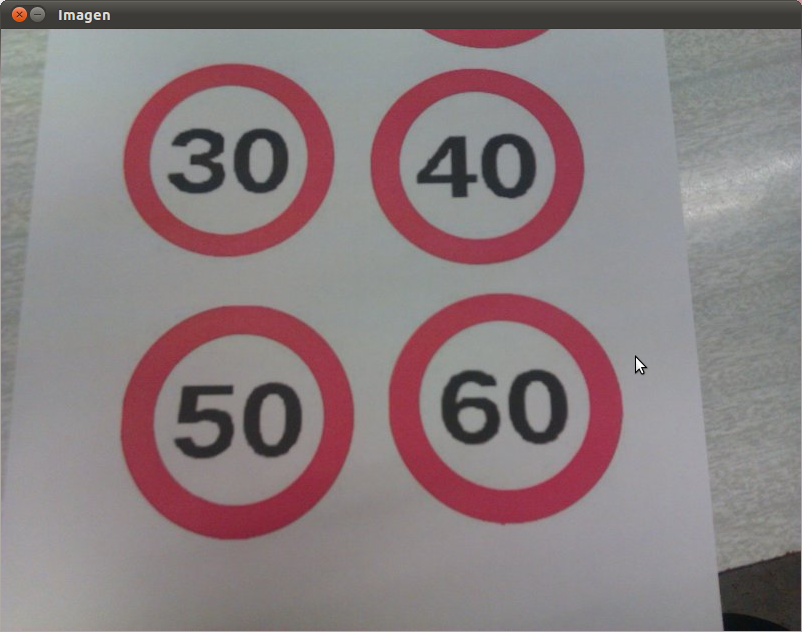
\includegraphics[width=7cm]{./imagenes/im-entrada.png} & 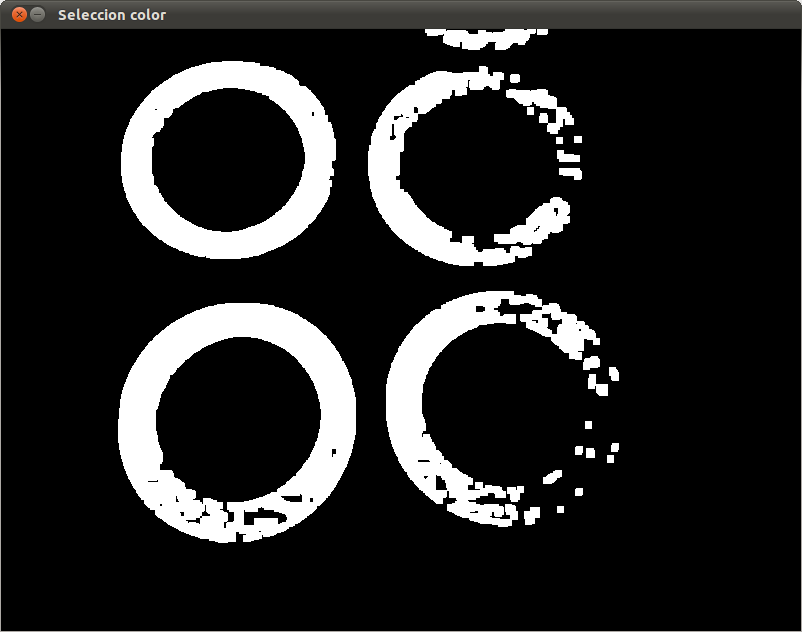
\includegraphics[width=7cm]{./imagenes/paso0.png}\\
        {Imagen de entrada (a).} & {Imagen resultante (b).}\\
      \end{tabular}
    \caption{Resultado de aplicar una selección por color sobre una imagen.}
    \label{fig:ejemplo-selec-color}
  \end{center}
\end{figure}

En la imagen \ref{fig:ejemplo-selec-color} de salida se puede apreciar un conjunto de objetos resultantes a los se les debe de aplicar algún mecanismo que permita trabajar con cada uno de los diferentes elementos por separado con la finalidad de poder clasificar cada uno de ellos de manera independiente.

\subsubsection {Extracción de objetos}
\label{sec:extraccion-objetos}

Una vez obtenida las agrupaciones de píxeles de tonalidad roja, figura \ref{fig:ejemplo-selec-color}, se procede a la identificación de cada una de esas agrupaciones por separado. Para ello utilizamos un método basado en la detección de contornos propio de OpenCV que está basado en el algoritmo de Canny. La aplicación de esta técnica nos permite averiguar los contornos de la imagen o, dicho de otro modo, los cambios bruscos de intensidades lumínicas.\\

Del paso anterior se obtiene una estructura tipo lista donde se encuentran almacenados todos los objetos detectados. El primer paso aplicado es descartar aquellos objetos cuyos valores de área son demasiado pequeños como para ser algunos de los elementos buscados, evitando así continuar con su análisis.\\

Los objetos restantes son, cada uno de ellos, encerrados dentro de una estructura rectangular de área mínima conociendo así su tamaño y coordenadas de localización.\\

Una vez conocidas las coordenadas que encierran al objeto, se establece una región de interés (ROI) en la imagen de entrada y en la obtenida tras la selección por color. Una región de interés es un área rectangular en una imagen, obteniendo el objeto segmentado para su posterior procesamiento. La figura \ref{fig:roi} muestra un claro ejemplo de una delimitación de una región de interés en una imagen.\\

\begin{figure}[H]
  \begin{center}
    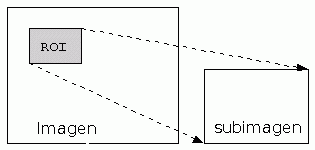
\includegraphics[scale=1]{roi.png}
  \end{center}
  \caption{Imagen con una región definida de interés.}
  \label{fig:roi}
\end{figure}

Cuando es asignada una región de interés en una imagen, todas las modificaciones realizadas sobre dicha imagen serán aplicadas sobre la zona seleccionada, una vez terminado el proceso de identificación del objeto encerrado en la región, ésta se libera y se procede a trabajar con una nueva región de interés en caso de existir más objetos candidatos a análisis en la imagen de entrada.\\

Una vez definidas las regiones de interés sobre ambas imágenes de la figura \ref{fig:ejemplo-selec-color}, se desea obtener la señal de forma independiente sin el fondo, para ello se emplea la técnica de copia usando una máscara, que no es más que copiar aquellos píxeles en una nueva imagen que se encuentren marcados en la imagen máscara. La imagen máscara es obtenida rellenando los huecos interiores de la imagen obtenida tras la aplicación de la selección por color. La figura \ref{fig:mascaras} muestra un ejemplo ilustrativo:\\

\begin{figure}[H]
  \begin{center}
      \begin{tabular}{ccc p{3cm}p{3cm}p{3cm}}
        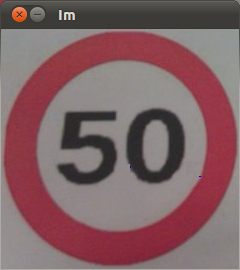
\includegraphics[width=3cm]{./imagenes/mascara/mascara1.png} &  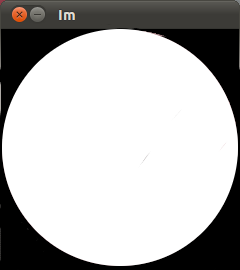
\includegraphics[width=3cm]{./imagenes/mascara/mascara2.png} & 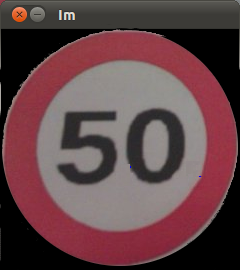
\includegraphics[width=3cm]{./imagenes/mascara/mascara3.png} \\
        {(\emph{a})} & {(\emph{b})} & {(\emph{c})} \\
      \end{tabular}
    \caption{Copia de una imagen mediante el uso de máscaras.}
    \label{fig:mascaras}
  \end{center}
\end{figure}

El código mostrado realiza las acciones de extracción de cada uno de los objetos por separado una vez aplicada la segmentación por color:\\

\underline{Código para la extracción de los objetos de una imagen}\\
\begin{Verbatim}[commandchars=\\\{\}]
\PY{c+c1}{// Segmentación por color}
\PY{n}{img\PYZus{}selec\PYZus{}color} \PY{o}{=} \PY{n}{segmentacion\PYZus{}RGB}\PY{p}{(}\PY{n}{img}\PY{p}{)}\PY{p}{;}

\PY{n}{dst} \PY{o}{=} \PY{n}{cvCreateImage}\PY{p}{(} \PY{n}{cvGetSize}\PY{p}{(}\PY{n}{img}\PY{p}{)}\PY{p}{,}\PY{n}{IPL\PYZus{}DEPTH\PYZus{}8U}\PY{p}{,} \PY{l+m+mi}{1} \PY{p}{)}\PY{p}{;}
\PY{n}{cvZero}\PY{p}{(}\PY{n}{dst}\PY{p}{)}\PY{p}{;}

\PY{c+c1}{// Búsqueda de contornos en la imagen obtenida tras la selección por color.}
\PY{n}{cvFindContours}\PY{p}{(}\PY{n}{img\PYZus{}selec\PYZus{}color}\PY{p}{,} \PY{n}{storage}\PY{p}{,} \PY{o}{&}\PY{n}{contour}\PY{p}{,} \PY{k}{sizeof}\PY{p}{(}\PY{n}{CvContour}\PY{p}{)}\PY{p}{,}
\PY{n}{CV\PYZus{}RETR\PYZus{}EXTERNAL}\PY{p}{,} \PY{n}{CV\PYZus{}CHAIN\PYZus{}APPROX\PYZus{}NONE}\PY{p}{)}\PY{p}{;}

\PY{n}{senial} \PY{o}{=} \PY{n}{cvCreateImage}\PY{p}{(}\PY{n}{cvGetSize}\PY{p}{(}\PY{n}{img}\PY{p}{)}\PY{p}{,} \PY{n}{IPL\PYZus{}DEPTH\PYZus{}8U}\PY{p}{,} \PY{l+m+mi}{3}\PY{p}{)}\PY{p}{;}
\PY{n}{cvZero}\PY{p}{(}\PY{n}{senial}\PY{p}{)}\PY{p}{;}     

\PY{c+c1}{// Para objeto encontrado:}
\PY{k}{for}\PY{p}{(}\PY{p}{;} \PY{n}{contour} \PY{o}{!}\PY{o}{=} \PY{l+m+mi}{0}\PY{p}{;} \PY{n}{contour} \PY{o}{=} \PY{n}{contour}\PY{o}{-}\PY{o}{>}\PY{n}{h\PYZus{}next} \PY{p}{)}\PY{p}{\PYZob{}}
  
  \PY{c+c1}{// Se calcula su área.}
  \PY{n}{area}\PY{o}{=}\PY{n}{fabs}\PY{p}{(}\PY{n}{cvContourArea}\PY{p}{(}\PY{n}{contour}\PY{p}{,}\PY{n}{CV\PYZus{}WHOLE\PYZus{}SEQ}\PY{p}{)}\PY{p}{)}\PY{p}{;}
  
  \PY{c+c1}{// Si el área supera un determinado valor de área. }
  \PY{k}{if}\PY{p}{(}\PY{n}{area}\PY{o}{>}\PY{o}{=}\PY{l+m+mi}{300}\PY{p}{)}\PY{p}{\PYZob{}}
    
    \PY{c+c1}{// Se dibuja el objeto en una imagen.}
    \PY{n}{cvDrawContours}\PY{p}{(}\PY{n}{dst}\PY{p}{,} \PY{n}{contour}\PY{p}{,} \PY{n}{cvScalar}\PY{p}{(}\PY{l+m+mi}{1}\PY{p}{)}\PY{p}{,}\PY{n}{cvScalar}\PY{p}{(}\PY{l+m+mi}{1}\PY{p}{)}\PY{p}{,} \PY{o}{-}\PY{l+m+mi}{1}\PY{p}{,} \PY{n}{CV\PYZus{}FILLED}\PY{p}{,} \PY{l+m+mi}{8}\PY{p}{)}\PY{p}{;}
    
    \PY{c+c1}{// Se calcula el área mínima que encierra al objeto.}
    \PY{n}{rect} \PY{o}{=} \PY{n}{cvBoundingRect}\PY{p}{(}\PY{n}{contour}\PY{p}{,}\PY{l+m+mi}{0}\PY{p}{)}\PY{p}{;} 
    
    \PY{c+c1}{// Selección de las regiones de interés.}
    \PY{n}{cvSetImageROI}\PY{p}{(}\PY{n}{dst}\PY{p}{,}\PY{n}{rect}\PY{p}{)}\PY{p}{;}
    \PY{n}{cvSetImageROI}\PY{p}{(}\PY{n}{senial}\PY{p}{,}\PY{n}{rect}\PY{p}{)}\PY{p}{;}
    \PY{n}{cvSetImageROI}\PY{p}{(}\PY{n}{img}\PY{p}{,}\PY{n}{rect}\PY{p}{)}\PY{p}{;}
    
    \PY{c+c1}{// Se realiza la copia mediante la}
    \PY{c+c1}{// utilización de máscaras para eliminar el fondo del objeto.}
    \PY{n}{cvCopy}\PY{p}{(}\PY{n}{img}\PY{p}{,}\PY{n}{senial}\PY{p}{,}\PY{n}{dst}\PY{p}{)}\PY{p}{;}

    \PY{c+c1}{// Se eliminan las regiones de interés establecidas previamente.}
    \PY{n}{cvResetImageROI}\PY{p}{(}\PY{n}{dst}\PY{p}{)}\PY{p}{;}
    \PY{n}{cvResetImageROI}\PY{p}{(}\PY{n}{img}\PY{p}{)}\PY{p}{;}
    
    \PY{c+c1}{// Se redimensiona la imagen.}
    \PY{n}{identificar} \PY{o}{=} \PY{n}{cvCreateImage}\PY{p}{(} \PY{n}{cvSize}\PY{p}{(}\PY{l+m+mi}{100}\PY{p}{,}\PY{l+m+mi}{100}\PY{p}{)}\PY{p}{,}\PY{n}{IPL\PYZus{}DEPTH\PYZus{}8U}\PY{p}{,}\PY{l+m+mi}{3}\PY{p}{)}\PY{p}{;}
    \PY{n}{cvResize}\PY{p}{(}\PY{n}{senial}\PY{p}{,}\PY{n}{identificar}\PY{p}{,}\PY{n}{CV\PYZus{}INTER\PYZus{}LINEAR}\PY{p}{)}\PY{p}{;}
    
    \PY{c+c1}{// Y ya disponemos la imagen con el elemento a identificar.   }
    \PY{n}{cvShowImage}\PY{p}{(} \PY{l+s}{"}\PY{l+s}{Elemento}\PY{l+s}{"}\PY{p}{,}\PY{n}{identificar}\PY{p}{)}\PY{p}{;}

    \PY{c+c1}{// ALGORITMO IDENTIFICADOR}

  \PY{p}{\PYZcb{}} \PY{c+c1}{// Fin if.}
 \PY{p}{\PYZcb{}} \PY{c+c1}{// Fin for.}
\end{Verbatim}


Una vez obtenida una imagen independiente con el objeto a identificar en color, imagen \emph{c} de la figura \ref{fig:mascaras} o la variable identificar del código anterior, debe ser redimensionada para que todos los objetos a análisis sean de igual tamaño para proceder a la aplicación de la técnica de clasificación denominada ``Template matching'' o comparación de plantillas.

\subsection {Template matching}

Para la identificación de los objetos en el primer prototipo se ha utilizado una técnica denominada Template Matching o comparación de plantillas.\\

Esta técnica consiste en la búsqueda de la región de una imagen que mayor semejanza guarda con la imagen dada como plantilla.\\

En la comparación de plantillas, todas las posibles localizaciones que pueden ser comparadas con la plantilla son almacenadas en una matriz \emph{R}, en la cual se almacenan los coeficientes resultantes de las comparaciones. El tamaño de la imagen de entrada es de \emph{W} x \emph{H} donde \emph{W} y \emph{H} representan el ancho y el alto de la imagen respectivamente y \emph{w} x \emph{h} se corresponde con el producto del ancho por el alto de la imagen plantilla. El tamaño de la matriz viene dado por $(W - w + 1) x (H - h + 1)$. \\

\begin{figure}[H]
  \begin{center}
    \begin{tabular}{cc p{6.6cm}p{8cm}}
      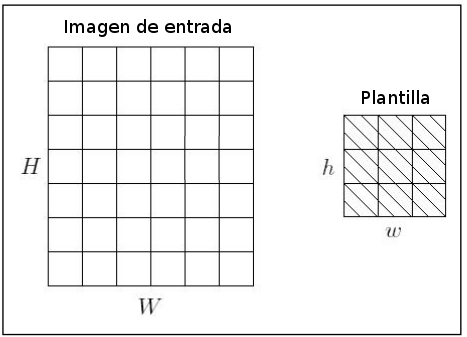
\includegraphics[width=6.6cm]{./imagenes/plantillas.png} &  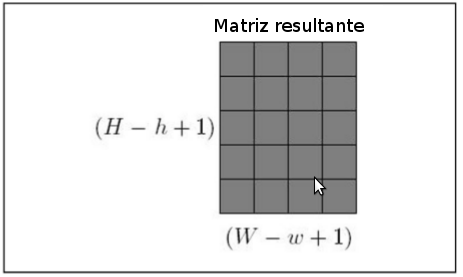
\includegraphics[width=8cm]{./imagenes/template-resultante.png} \\
                      {Matrices de origen (\emph{a}).} & {Matriz resultado (\emph{b}).} \\
    \end{tabular}
  \end{center}
  \caption{Matrices de entrada y de salida para la técnica de comparación de plantillas.}
\end{figure}
  \label{fig:template-in-out}

\begin{figure}[H]
  \begin{center}
    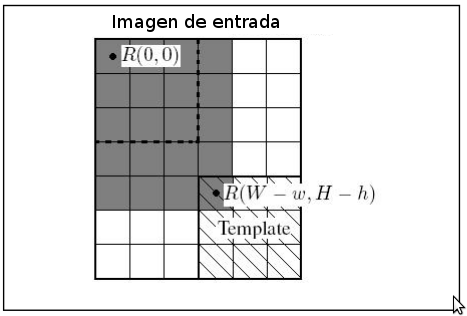
\includegraphics[scale=0.6]{ejemplo-template.png}
  \end{center}
  \caption{El valor de cada píxel de la posición $(x,y)$ es procesado para obtener su característica de similitud entre la plantilla y el rectángulo resultante de tomar $(x,y)$ como píxel situado en la esquina superior izquierda.}
  \label{fig:template}
\end{figure}

Las referencias del tamaño y la representación del proceso de comparación de plantillas se muestra en las figuras \ref{fig:template-in-out} (a) y \ref{fig:template}, respectivamente.\\

La figura \ref{fig:template-in-out} (b), muestra la matriz final obtenida tras el proceso de búsqueda de una plantilla en una imagen.\\

Existen varios métodos para la comparación de plantillas, algunos de los más conocidos son la suma de las diferencias al cuadrado, correlación cruzada y el método del Coeficiente de Correlación. Dependiendo del algoritmo, el resultado correspondiente puede ser ligeramente diferente. Se considera \emph{T} como la imagen de la plantilla e \emph{I} como la imagen de entrada. En el presente prototipo el método de las diferencias al cuadrado es el que ha resultado más eficaz. A continuación se muestra su fundamento matemático:\\

\begin{equation}
  R(x,y) = \frac{\sum_{x',y'} (T(x',y') - I(x+x',y+y'))^2} {\sqrt{\sum_{x',y'}T(x',y')^2 \cdot \sum_{x',y'}I(x+x',y+y')}} 
\label{eq:template-def}
\end{equation}

Los valores obtenidos tras aplicar \ref{eq:template-def} en cada píxel de la imagen de entrada son almacenados en una matriz de salida \emph{R} anteriormente descrita. Dicha matriz finalmente se recorre localizando aquellos valores que superen un umbral fijado con el fin de dar por localizado el objeto que se encontraba en la imagen que ha sido empleada como plantilla.\\
  
A continuación se muestra el código realizado en OpenCV para la comparación de plantillas:\\

\underline{Código para la detección de un objeto}\\
\begin{Verbatim}[commandchars=\\\{\}]
\PY{c+c1}{// ALGORITMO DE IDENTIFICACIÓN}

\PY{c+c1}{// Carga de imagen referencia o plantilla.}
\PY{n}{tpl} \PY{o}{=} \PY{n}{cvLoadImage}\PY{p}{(} \PY{n}{directorio}\PY{p}{,} \PY{n}{CV\PYZus{}LOAD\PYZus{}IMAGE\PYZus{}COLOR} \PY{p}{)}\PY{p}{;}

\PY{c+c1}{// Cáculo de ancho y alto de la imagen resultado.}
\PY{n}{width}  \PY{o}{=} \PY{n}{identificar}\PY{o}{-}\PY{o}{>}\PY{n}{width}  \PY{o}{-} \PY{n}{tpl}\PY{o}{-}\PY{o}{>}\PY{n}{width} \PY{o}{+} \PY{l+m+mi}{1}\PY{p}{;}
\PY{n}{height} \PY{o}{=} \PY{n}{identificar}\PY{o}{-}\PY{o}{>}\PY{n}{height} \PY{o}{-} \PY{n}{tpl}\PY{o}{-}\PY{o}{>}\PY{n}{height} \PY{o}{+} \PY{l+m+mi}{1}\PY{p}{;}

\PY{c+c1}{// Se crea la imagen donde se almacenará el resultado de la comparación.}
\PY{n}{res} \PY{o}{=} \PY{n}{cvCreateImage}\PY{p}{(} \PY{n}{cvSize}\PY{p}{(} \PY{n}{width}\PY{p}{,} \PY{n}{height} \PY{p}{)}\PY{p}{,} \PY{n}{IPL\PYZus{}DEPTH\PYZus{}32F}\PY{p}{,} \PY{l+m+mi}{1} \PY{p}{)}\PY{p}{;}

\PY{c+c1}{// Se realiza la comparación:}
\PY{n}{cvMatchTemplate}\PY{p}{(}\PY{n}{identificar}\PY{p}{,} \PY{n}{tpl}\PY{p}{,} \PY{n}{res}\PY{p}{,} \PY{n}{CV\PYZus{}TM\PYZus{}SQDIFF\PYZus{}NORMED}\PY{p}{)}\PY{p}{;}

\PY{k}{for}\PY{p}{(} \PY{n}{i} \PY{o}{=} \PY{l+m+mi}{0} \PY{p}{;} \PY{n}{i} \PY{o}{<} \PY{n}{height} \PY{p}{;} \PY{n}{i}\PY{o}{+}\PY{o}{+}\PY{p}{)} \PY{p}{\PYZob{}}
  \PY{k}{for}\PY{p}{(} \PY{n}{j} \PY{o}{=} \PY{l+m+mi}{0} \PY{p}{;} \PY{n}{j} \PY{o}{<} \PY{n}{width} \PY{p}{;} \PY{n}{j}\PY{o}{+}\PY{o}{+}\PY{p}{)} \PY{p}{\PYZob{}}

    \PY{c+c1}{// sacamos el elemento:}
    \PY{n}{s} \PY{o}{=} \PY{n}{cvGet2D}\PY{p}{(} \PY{n}{res}\PY{p}{,} \PY{n}{i}\PY{p}{,} \PY{n}{j} \PY{p}{)}\PY{p}{;}
    
    \PY{c+c1}{// Si el valor se localiza entre el rango establecido...}
    \PY{k}{if}\PY{p}{(} \PY{n}{s}\PY{p}{.}\PY{n}{val}\PY{p}{[}\PY{l+m+mi}{0}\PY{p}{]} \PY{o}{<}\PY{o}{=} \PY{n}{umbral} \PY{p}{)} \PY{p}{\PYZob{}}
      \PY{c+c1}{// Dibujamos el contorno al objeto identificado ENCONTRADO!}
      \PY{n}{fprintf}\PY{p}{(} \PY{n}{stderr}\PY{p}{,} \PY{l+s}{"}\PY{l+s}{¡50 m/h!}\PY{l+s}{"}\PY{p}{)}\PY{p}{;}
      
      \PY{n}{pt1}\PY{p}{.}\PY{n}{x} \PY{o}{=} \PY{n}{rect}\PY{p}{.}\PY{n}{x}\PY{p}{;}
      \PY{n}{pt1}\PY{p}{.}\PY{n}{y} \PY{o}{=} \PY{n}{rect}\PY{p}{.}\PY{n}{y}\PY{p}{;}
      \PY{n}{pt2}\PY{p}{.}\PY{n}{x} \PY{o}{=} \PY{n}{rect}\PY{p}{.}\PY{n}{x} \PY{o}{+} \PY{n}{rect}\PY{p}{.}\PY{n}{width}\PY{p}{;}
      \PY{n}{pt2}\PY{p}{.}\PY{n}{y} \PY{o}{=} \PY{n}{rect}\PY{p}{.}\PY{n}{y} \PY{o}{+} \PY{n}{rect}\PY{p}{.}\PY{n}{height}\PY{p}{;}
      
      \PY{c+c1}{// Se dibuja el rectángulo que encierra al objeto.}
      \PY{n}{cvRectangle}\PY{p}{(}\PY{n}{img}\PY{p}{,}\PY{n}{pt1}\PY{p}{,}\PY{n}{pt2}\PY{p}{,}\PY{n}{CV\PYZus{}RGB}\PY{p}{(}\PY{l+m+mi}{0}\PY{p}{,}\PY{l+m+mi}{255}\PY{p}{,}\PY{l+m+mi}{0}\PY{p}{)}\PY{p}{,}\PY{l+m+mi}{3}\PY{p}{,}\PY{l+m+mi}{8}\PY{p}{,}\PY{l+m+mi}{0}\PY{p}{)}\PY{p}{;}
    \PY{p}{\PYZcb{}}
  \PY{p}{\PYZcb{}}
 \PY{p}{\PYZcb{}}
\end{Verbatim}


La figura \ref{fig:detectado} muestra una imagen donde se aprecia cómo el objeto utilizado como plantilla ha sido detectado:\\

\begin{figure}[H]
  \begin{center}
    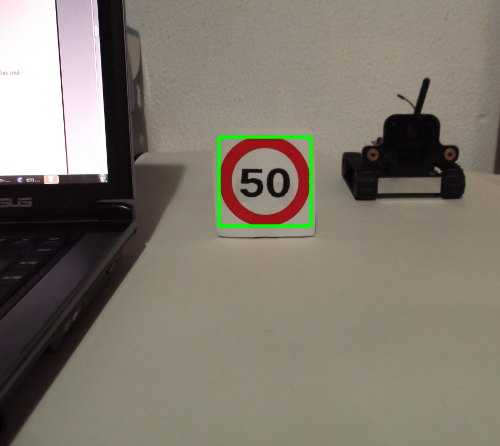
\includegraphics[scale=0.5]{detectado2.png}
  \end{center}
  \caption{Vista de la señal detectada en la imagen.}
  \label{fig:detectado}
\end{figure}

La técnica de comparación de plantillas, como se ha descrito, presenta la particularidad de encontrar un determinado objeto dentro de una imagen, por tanto, a priori el preprocesado previo realizado para aplicar una segmentación por color y extracción de los objetos por separado antes de emplear este algoritmo de clasificación no resulta necesario para su funcionamiento. El preprocesado previo se ha realizado para evitar las innecesarias comparaciones en zonas de la imagen donde sabemos que el objeto buscado no se va a encontrar, ganando por tanto en eficiencia.

\subsection{Problemas detectados}

Los problemas que han llevado a cabo el rechazo de este primer prototipo han sido los siguientes:

\begin{itemize}

\item El problema de la utilización de una segmentación por color siguiendo el modelo RGB es que sufre una extrema sensibilidad de variación de los valores de un determinado color a las condiciones lumínicas del entorno. Esto ocasiona que el prototipo desarrollado solo sea funcional en un único entorno, por ejemplo, la sala donde se ha desarrollado y probado, dejando de ser funcional en otras situaciones y lugares siendo necesario idear una nueva metodología de segmentación para el siguiente prototipo.

\item El problema del Template Matching es que ha de comparar muchas características (para él, un píxel es una característica), y si tenemos en cuenta que en la base de datos encontramos N señales, observamos que este método el resultado no ofrece garantías de funcionamiento en tiempo real, condición indispensable del proyecto.

\end{itemize}

\section{Segundo prototipo}

Este segundo prototipo difiere del anterior por la utilización para la segmentación por color del modelo de color HSV. Este modelo de color es mucho menos sensible a las condiciones lumínicas del entorno, permitiendo la detección de las tonalidades deseadas en situaciones donde el primer prototipo presentaba problemas.\\

Por otro lado, para la clasificación se ha optado por la utilización del algoritmo de los K-vecinos en lugar de la comparación de plantillas o Template Matching.\\

Destacar que para la función del algoritmo de los k-vecinos resulta necesaria una recolección previa de los datos de los elementos a detectar, los denominados clases, con el fin de realizar una serie de comparaciones entre el objeto desconocido y los datos previamente extraídos con la finalidad de determinar a que clase corresponde. Por tanto se describirá el algoritmo de entrenamiento (extracción de datos) y el algoritmo de detección (clasificación) utilizados.

\subsection{Extracción de características}

Para poder clasificar satisfactoriamente los elementos, es necesario un proceso de aprendizaje previo en el cual el sistema crea un modelo de cada una de las clases a partir de una secuencia de entrenamiento o conjunto de vectores de características de cada una de las clases.\\

Debido a esta razón, debemos previamente, antes de realizar cualquier tarea de clasificación, elaborar un conjunto de vectores de características o también denominado matriz de modelos con el fin de cotejar las características del elemento a identificar con los datos de la matriz modelos. A la fase de obtención de la matriz de modelos se le denomina etapa de entrenamiento en un sistema de reconocimiento de patrones. Dicha matriz ha sido obtenida en una serie de etapas que se describen en los sucesivos puntos de esta sección. 

\subsubsection {Segmentación por color siguiendo el modelo HSV}
\label{sec:color-HSV}

En la primera etapa del entrenamiento se ha optado por continuar con una técnica de segmentación por color, pero en esta ocasión siguiendo el modelo HSV. Cabe recordar que la finalidad de la segmentación es la de realizar una correcta selección de aquellos píxeles que según una determinada tonalidad resultan útiles para el posterior procesamiento e identificación de objetos.\\

En esta ocasión se presenta el mismo problema que con el primer prototipo, se desconocen los valores correspondiente al color a identificar, siendo, de igual modo, necesario conocer las tonalidades exactas y cómo la susodicha tonalidad es representada por el ordenador. La solución en este caso fue adaptar la herramienta empleada en el primer prototipo. Dicha herramienta mostraba el valor de un determinado píxel al pulsar sobre el mismo, solo que en esta ocasión en formato HSV.  El código del programa es idéntico al mostrado en el primer prototipo pero realizando previamente una transformación de la imagen del formato RGB al formato HSV.\\

 En la figura \ref{fig:color-pixel2} se puede observar el funcionamiento del programa mostrando el color sobre el que se ha hecho click, apreciándose como el último color seleccionado posee los valores en sus tres canales: Hue, Saturation, Value, en castellano, tono, saturación y valor. Los valores obtenidos son (175,52,220) fijándonos en los valores correspondientes al tono y la saturación. El programa se escribió en lenguaje C haciendo uso de la biblioteca OpenCV.\\

\begin{figure}[H]
  \begin{center}
    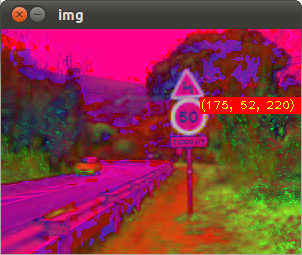
\includegraphics[scale=0.7]{color-pixel2.png}
  \end{center}
  \caption{Programa elaborado para la obtención de los valores del píxel pulsado.}
  \label{fig:color-pixel2}
\end{figure}

La aplicación de este modelo resulta mucho más ventajosa con respecto al modelo RGB debido a que HSV sólo precisa de un solo valor numérico para detectar el color, desde tonos relativamente ligeros hasta los tonos más oscuros. La cantidad de color y el brillo del color son manejados por la \emph{saturación} y los parámetros \emph{valor}, respectivamente.\\

A continuación se muestra el código realizado para realizar la segmentación por color de una imagen de entrada, en la cual, al igual que la función desarrollada para la segmentación siguiendo el modelo RGB, se han fijado unos umbrales y se ha recorrido la imagen identificando aquellos píxeles que cumplen las condiciones dejando el píxel activado en una imagen de salida.\\

\underline{Segmentación de una imagen siguiendo el modelo de color HSV}\\
\begin{Verbatim}[commandchars=\\\{\}]
\PY{n}{IplImage}\PY{o}{*} \PY{n}{seleccion\PYZus{}colorHSV}\PY{p}{(}\PY{n}{IplImage}\PY{o}{*} \PY{n}{img} \PY{p}{)}\PY{p}{\PYZob{}}

  \PY{c+c1}{// Declaración de variables}
  \PY{n}{IplImage} \PY{o}{*}\PY{n}{hsv\PYZus{}Image}\PY{p}{,} \PY{o}{*}\PY{n}{mono\PYZus{}Image}\PY{p}{;}
  \PY{k+kt}{int} \PY{n}{height} \PY{p}{,} \PY{n}{width} \PY{p}{,} \PY{n}{step} \PY{p}{,} \PY{n}{channels}\PY{p}{;}
  \PY{k+kt}{int} \PY{n}{step\PYZus{}mono} \PY{p}{,} \PY{n}{channels\PYZus{}mono}\PY{p}{;}  
  \PY{n}{uchar} \PY{o}{*}\PY{n}{data\PYZus{}hsv} \PY{p}{,} \PY{o}{*}\PY{n}{data\PYZus{}mono}\PY{p}{;}


  \PY{c+c1}{// Declaración de los valores umbral.}
  \PY{k+kt}{int} \PY{n}{hupper}\PY{o}{=}\PY{l+m+mi}{175}\PY{p}{,}\PY{n}{hlower}\PY{o}{=}\PY{l+m+mi}{110}\PY{p}{,}\PY{n}{Saturation}\PY{o}{=}\PY{l+m+mi}{60}\PY{p}{,}\PY{n}{Brightness}\PY{o}{=}\PY{l+m+mi}{90}\PY{p}{,}\PY{n}{Erode}\PY{o}{=}\PY{l+m+mi}{1}\PY{p}{,}\PY{n}{Dilate}\PY{o}{=}\PY{l+m+mi}{1}\PY{p}{;}

  \PY{k+kt}{int} \PY{n}{hupper2}\PY{o}{=}\PY{l+m+mi}{35}\PY{p}{,}\PY{n}{hlower2}\PY{o}{=}\PY{l+m+mi}{0}\PY{p}{,}\PY{n}{Saturation2}\PY{o}{=}\PY{l+m+mi}{60}\PY{p}{,}\PY{n}{Brightness2}\PY{o}{=}\PY{l+m+mi}{60}\PY{p}{,}\PY{n}{Erode2}\PY{o}{=}\PY{l+m+mi}{0}\PY{p}{,}\PY{n}{Dilate2}\PY{o}{=}\PY{l+m+mi}{3}\PY{p}{;}   
  \PY{c+c1}{//}

  \PY{c+c1}{// Se crean dos imágenes del tamaño de la imagen fuente.}
  \PY{n}{hsv\PYZus{}Image} \PY{o}{=} \PY{n}{cvCreateImage}\PY{p}{(} \PY{n}{cvGetSize}\PY{p}{(}\PY{n}{img}\PY{p}{)}\PY{p}{,} \PY{l+m+mi}{8}\PY{p}{,} \PY{l+m+mi}{3} \PY{p}{)}\PY{p}{;}
  \PY{n}{mono\PYZus{}Image} \PY{o}{=} \PY{n}{cvCreateImage}\PY{p}{(} \PY{n}{cvGetSize}\PY{p}{(}\PY{n}{img}\PY{p}{)}\PY{p}{,} \PY{l+m+mi}{8}\PY{p}{,} \PY{l+m+mi}{1} \PY{p}{)}\PY{p}{;}
  \PY{c+c1}{// Se inicializan a cero.}
  \PY{n}{cvZero}\PY{p}{(}\PY{n}{hsv\PYZus{}Image}\PY{p}{)}\PY{p}{;}
  \PY{n}{cvZero}\PY{p}{(}\PY{n}{mono\PYZus{}Image}\PY{p}{)}\PY{p}{;}

  \PY{c+c1}{// Obtenemos atributos de la imagen HSV.}
  \PY{n}{height}     \PY{o}{=} \PY{n}{hsv\PYZus{}Image}\PY{o}{-}\PY{o}{>}\PY{n}{height}\PY{p}{;}
  \PY{n}{width}      \PY{o}{=} \PY{n}{hsv\PYZus{}Image}\PY{o}{-}\PY{o}{>}\PY{n}{width}\PY{p}{;}
  \PY{n}{step}       \PY{o}{=} \PY{n}{hsv\PYZus{}Image}\PY{o}{-}\PY{o}{>}\PY{n}{widthStep}\PY{o}{/}\PY{k}{sizeof}\PY{p}{(}\PY{n}{uchar}\PY{p}{)}\PY{p}{;}
  \PY{n}{channels}   \PY{o}{=} \PY{n}{hsv\PYZus{}Image}\PY{o}{-}\PY{o}{>}\PY{n}{nChannels}\PY{p}{;}
  \PY{n}{step\PYZus{}mono}   \PY{o}{=} \PY{n}{mono\PYZus{}Image}\PY{o}{-}\PY{o}{>}\PY{n}{widthStep}\PY{o}{/}\PY{k}{sizeof}\PY{p}{(}\PY{n}{uchar}\PY{p}{)}\PY{p}{;}
  \PY{n}{channels\PYZus{}mono} \PY{o}{=} \PY{n}{mono\PYZus{}Image}\PY{o}{-}\PY{o}{>}\PY{n}{nChannels}\PY{p}{;}

  \PY{c+c1}{// Convertimos imagen de entrada de RGB a HSV.}
  \PY{n}{cvCvtColor}\PY{p}{(}\PY{n}{img}\PY{p}{,}\PY{n}{hsv\PYZus{}Image}\PY{p}{,}\PY{n}{CV\PYZus{}RGB2HSV}\PY{p}{)}\PY{p}{;}

  \PY{c+c1}{// Obtenemos los valores RGB de la Imagen.}
  \PY{n}{data\PYZus{}hsv} \PY{o}{=} \PY{p}{(}\PY{n}{uchar} \PY{o}{*}\PY{p}{)}\PY{n}{hsv\PYZus{}Image}\PY{o}{-}\PY{o}{>}\PY{n}{imageData}\PY{p}{;}
  \PY{n}{data\PYZus{}mono} \PY{o}{=} \PY{p}{(}\PY{n}{uchar} \PY{o}{*}\PY{p}{)}\PY{n}{mono\PYZus{}Image}\PY{o}{-}\PY{o}{>}\PY{n}{imageData}\PY{p}{;}

  \PY{c+c1}{//Recorremos la imagen.}
  \PY{k}{for}\PY{p}{(}\PY{k+kt}{int} \PY{n}{i} \PY{o}{=} \PY{l+m+mi}{0}\PY{p}{;} \PY{n}{i} \PY{o}{<}\PY{n}{height}\PY{p}{;} \PY{n}{i}\PY{o}{+}\PY{o}{+} \PY{p}{)} \PY{p}{\PYZob{}}
    \PY{k}{for}\PY{p}{(}\PY{k+kt}{int} \PY{n}{j} \PY{o}{=} \PY{l+m+mi}{0}\PY{p}{;} \PY{n}{j} \PY{o}{<}\PY{n}{width}\PY{p}{;} \PY{n}{j}\PY{o}{+}\PY{o}{+} \PY{p}{)} \PY{p}{\PYZob{}}

        \PY{c+c1}{// Segmentamos la imagen mediante los valores umbrales }
        \PY{c+c1}{// correspondientes al color rojo y azul.}
        \PY{k}{if} \PY{p}{(}\PY{p}{(}\PY{p}{(}\PY{n}{data\PYZus{}hsv}\PY{p}{[}\PY{n}{i}\PY{o}{*}\PY{n}{step}\PY{o}{+}\PY{n}{j}\PY{o}{*}\PY{n}{channels}\PY{p}{]}\PY{p}{)}\PY{o}{>}\PY{o}{=} \PY{n}{hlower}\PY{p}{)} \PY{o}{&}\PY{o}{&}
            \PY{p}{(}\PY{p}{(}\PY{n}{data\PYZus{}hsv}\PY{p}{[}\PY{n}{i}\PY{o}{*}\PY{n}{step}\PY{o}{+}\PY{n}{j}\PY{o}{*}\PY{n}{channels}\PY{p}{]}\PY{p}{)} \PY{o}{<}\PY{o}{=} \PY{n}{hupper}\PY{p}{)} \PY{o}{&}\PY{o}{&} 
            \PY{p}{(}\PY{n}{data\PYZus{}hsv}\PY{p}{[}\PY{n}{i}\PY{o}{*}\PY{n}{step}\PY{o}{+}\PY{n}{j}\PY{o}{*}\PY{n}{channels}\PY{o}{+}\PY{l+m+mi}{1}\PY{p}{]}\PY{o}{>}\PY{o}{=} \PY{n}{Saturation} \PY{p}{)} \PY{o}{&}\PY{o}{&} 
            \PY{p}{(}\PY{n}{data\PYZus{}hsv}\PY{p}{[}\PY{n}{i}\PY{o}{*}\PY{n}{step}\PY{o}{+}\PY{n}{j}\PY{o}{*}\PY{n}{channels}\PY{o}{+}\PY{l+m+mi}{2}\PY{p}{]}\PY{o}{>}\PY{o}{=} \PY{n}{Brightness}\PY{p}{)} \PY{o}{|}\PY{o}{|} 
            \PY{p}{(}\PY{p}{(}\PY{n}{data\PYZus{}hsv}\PY{p}{[}\PY{n}{i}\PY{o}{*}\PY{n}{step}\PY{o}{+}\PY{n}{j}\PY{o}{*}\PY{n}{channels}\PY{p}{]}\PY{p}{)}\PY{o}{>}\PY{o}{=} \PY{n}{hlower2}\PY{p}{)} \PY{o}{&}\PY{o}{&}
            \PY{p}{(}\PY{p}{(}\PY{n}{data\PYZus{}hsv}\PY{p}{[}\PY{n}{i}\PY{o}{*}\PY{n}{step}\PY{o}{+}\PY{n}{j}\PY{o}{*}\PY{n}{channels}\PY{p}{]}\PY{p}{)} \PY{o}{<}\PY{o}{=} \PY{n}{hupper2}\PY{p}{)} \PY{o}{&}\PY{o}{&} 
            \PY{p}{(}\PY{n}{data\PYZus{}hsv}\PY{p}{[}\PY{n}{i}\PY{o}{*}\PY{n}{step}\PY{o}{+}\PY{n}{j}\PY{o}{*}\PY{n}{channels}\PY{o}{+}\PY{l+m+mi}{1}\PY{p}{]}\PY{o}{>}\PY{o}{=} \PY{n}{Saturation2} \PY{p}{)} \PY{o}{&}\PY{o}{&} 
            \PY{p}{(}\PY{n}{data\PYZus{}hsv}\PY{p}{[}\PY{n}{i}\PY{o}{*}\PY{n}{step}\PY{o}{+}\PY{n}{j}\PY{o}{*}\PY{n}{channels}\PY{o}{+}\PY{l+m+mi}{2}\PY{p}{]}\PY{o}{>}\PY{o}{=} \PY{n}{Brightness2}\PY{p}{)}\PY{p}{)}\PY{p}{\PYZob{}}

             \PY{c+c1}{// Coloreamos el píxel deseado en la }
             \PY{c+c1}{// imagen de salida.}
             \PY{n}{data\PYZus{}mono}\PY{p}{[}\PY{n}{i}\PY{o}{*}\PY{n}{step\PYZus{}mono}\PY{o}{+}\PY{n}{j}\PY{o}{*}\PY{n}{channels\PYZus{}mono}\PY{p}{]} \PY{o}{=} \PY{l+m+mi}{1}\PY{p}{;}
      \PY{p}{\PYZcb{}}
    \PY{p}{\PYZcb{}}
  \PY{p}{\PYZcb{}}

  \PY{c+c1}{// Se aplica una erosión y una dilatación,}
  \PY{c+c1}{// para la eliminacion de píxeles sueltos.}
  \PY{n}{cvErode}\PY{p}{(}\PY{n}{mono\PYZus{}Image}\PY{p}{,}\PY{n}{mono\PYZus{}Image}\PY{p}{,}\PY{l+m+mi}{0}\PY{p}{,}\PY{n}{Erode}\PY{p}{)}\PY{p}{;}
  \PY{n}{cvDilate}\PY{p}{(} \PY{n}{mono\PYZus{}Image}\PY{p}{,}\PY{n}{mono\PYZus{}Image}\PY{p}{,}\PY{l+m+mi}{0}\PY{p}{,}\PY{n}{Dilate}\PY{p}{)}\PY{p}{;}

  \PY{c+c1}{// Eliminación de estructuras innecesarias.}
  \PY{n}{cvReleaseImage}\PY{p}{(}\PY{o}{&}\PY{n}{hsv\PYZus{}Image}\PY{p}{)}\PY{p}{;}

  \PY{c+c1}{// Devolución de la imagen de salida.}
  \PY{k}{return} \PY{n}{mono\PYZus{}Image}\PY{p}{;}
\PY{p}{\PYZcb{}}
\end{Verbatim}



\subsubsection{Extracción de objetos}

Una vez obtenida la imagen con los píxeles seleccionados, el proceso de extracción de cada uno de los objetos y su análisis por separado se ha realizado de modo idéntico al utilizado en el primer prototipo. Ver sección \ref{sec:extraccion-objetos}.

\subsubsection {Obtención de datos representativos}

Una vez aplicada la segmentación por color siguiendo el modelo de color HSV, disponemos una nueva imagen la cual presenta unas agrupaciones de píxeles que han resultado seleccionados de la etapa anterior. Esas agrupaciones de píxeles son los objetos  que pasaremos a extraer sus características, que en nuestro caso son objetos que conocemos a que clase pertenecen y que deberemos de aplicar un procesamiento con el fin de extraer los datos y almacenarlos en la matriz modelos.\\

En esta ocasión, a diferencia del primer prototipo, en vez de aplicar la comparación de plantillas, se utilizará la matriz de modelos con aquellos datos que resulten identificativos de las clases. Dicha matriz tiene como objetivo proporcionar información de las diferentes señales de tráfico siendo un medio para cotejar los datos de un elemento desconocido y llevar a cabo su posterior clasificación.\\

Entre los datos extraídos disponemos:

\begin{itemize}
\item Forma de la figura:
  \begin{itemize}
  \item Círculo.
  \item Octógono.
  \end{itemize}
\item Perímetro del objeto/s interior/es.
\item Área del objeto/s interior/es.
\item Número de piezas interiores.
\item Número de vértices de las figuras interiores.
\end{itemize}

A continuación se describe la metodología seguida para el cálculo de los datos anteriormente enumerados:\\

\textbf{Forma de la figura:}
Se consideró necesario la realización de un algoritmo para la identificación de las formas externas de los objetos a ser analizados con el fin de poder distinguir correctamente entre los objetos circulares y octogonales, que son las que reconocerá el sistema. Aunque el algoritmo desarrollado también se ha desarrollado para la detección de formas triangulares y cuadradas.\\

Para la detección de circunferencias se ha empleado un algoritmo denominado la Transformada de Hough, el cual es incorporado en la biblioteca OpenCV. Este algoritmo es ampliamente utilizado en reconocimiento de patrones en imágenes ya que permite encontrar ciertas formas dentro de una imagen, como líneas, círculos, etc. \\

El algoritmo es aplicable a una imagen binarizada obtenida tras la realización de una detección de bordes devolviendo el número de círculos y su secuencia de puntos de cada uno de ellos.\\

Se consulta el radio de cada círculo y nos quedamos con el mayor, si el radio es de una tamaño considerable, se acepta la figura como un círculo.\\

Para la detección de las figuras octogonales se ha procedido a calcular mediante las funciones propias de la biblioteca OpenCV, obteniendo el polígono aproximado de tamaño mínimo que encierra la figura y consultando su número de vértices. Si dicho número se corresponde con ocho se procede a calcular el ángulo de cada uno de esos vértices.\\

Para ello se ha desarrollado la siguiente función:\\

\underline{Cálculo del ángulo entre dos vectores}\\
\begin{Verbatim}[commandchars=\\\{\}]
\PY{k+kt}{double} \PY{n+nf}{angulo}\PY{p}{(} \PY{n}{CvPoint}\PY{o}{*} \PY{n}{pt1}\PY{p}{,} \PY{n}{CvPoint}\PY{o}{*} \PY{n}{pt2}\PY{p}{,} \PY{n}{CvPoint}\PY{o}{*} \PY{n}{pt0} \PY{p}{)}
\PY{p}{\PYZob{}}
    \PY{k+kt}{double} \PY{n}{dx1} \PY{o}{=} \PY{n}{pt1}\PY{o}{-}\PY{o}{>}\PY{n}{x} \PY{o}{-} \PY{n}{pt0}\PY{o}{-}\PY{o}{>}\PY{n}{x}\PY{p}{;}
    \PY{k+kt}{double} \PY{n}{dy1} \PY{o}{=} \PY{n}{pt1}\PY{o}{-}\PY{o}{>}\PY{n}{y} \PY{o}{-} \PY{n}{pt0}\PY{o}{-}\PY{o}{>}\PY{n}{y}\PY{p}{;}
    \PY{k+kt}{double} \PY{n}{dx2} \PY{o}{=} \PY{n}{pt2}\PY{o}{-}\PY{o}{>}\PY{n}{x} \PY{o}{-} \PY{n}{pt0}\PY{o}{-}\PY{o}{>}\PY{n}{x}\PY{p}{;}
    \PY{k+kt}{double} \PY{n}{dy2} \PY{o}{=} \PY{n}{pt2}\PY{o}{-}\PY{o}{>}\PY{n}{y} \PY{o}{-} \PY{n}{pt0}\PY{o}{-}\PY{o}{>}\PY{n}{y}\PY{p}{;}

    \PY{k}{return} \PY{p}{(}\PY{p}{(}\PY{n}{dx1}\PY{o}{*}\PY{n}{dx2} \PY{o}{+} \PY{n}{dy1}\PY{o}{*}\PY{n}{dy2}\PY{p}{)}\PY{o}{/}\PY{n}{sqrt}\PY{p}{(}\PY{p}{(}\PY{n}{dx1}\PY{o}{*}\PY{n}{dx1} \PY{o}{+} \PY{n}{dy1}\PY{o}{*}\PY{n}{dy1}\PY{p}{)}\PY{o}{*}
            \PY{p}{(}\PY{n}{dx2}\PY{o}{*}\PY{n}{dx2} \PY{o}{+} \PY{n}{dy2}\PY{o}{*}\PY{n}{dy2}\PY{p}{)} \PY{o}{+} \PY{l+m+mf}{1e-10}\PY{p}{)}\PY{p}{;}
\PY{p}{\PYZcb{}}
\end{Verbatim}


La función calcula el ángulo de dos vectores obtenidos a partir de las coordenadas de entrada. La fórmula para calcular el ángulo entre dos vectores es la siguiente:\\\\

\begin{figure}[H]
  \begin{center}
    \[
      \cos \alpha = \frac{u_1 \cdot v_1 + u_2 \cdot v_2}{ \sqrt{u_1^2 + u_2^2} \cdot \sqrt{v_1^2 + v_2^2}}
      \nocite{}
    \]
  \end{center}
  \label{eq:angulo-vect}
  \caption{Fórmula para el cálculo del ángulo entre dos vectores.}
\end{figure}

Si los ángulos obtenidos, valor de $\alpha$, para cada vértice se sitúan en torno a los 45$^\circ$ se determina el objeto como un octógono.\\

A continuación se añade el código para la detección de las formas de las figuras, la cual realiza la llamada a la función ángulo antes mencionada.\\


\underline{Código para el cálculo del ángulo entre dos rectas dadas tres coordenadas}\\

\begin{Verbatim}[commandchars=\\\{\}]
\PY{c+c1}{//Localiza la forma de la figura a partir de un polígono.}

\PY{k+kt}{int} \PY{n}{tipo\PYZus{}figura}\PY{p}{(}\PY{n}{CvSeq}\PY{o}{*} \PY{n}{result}\PY{p}{,}\PY{n}{IplImage}\PY{o}{*} \PY{n}{plantilla}\PY{p}{)}\PY{p}{\PYZob{}}  

  \PY{k+kt}{double} \PY{n}{PI} \PY{o}{=} \PY{l+m+mf}{3.1415}\PY{p}{;}

  \PY{k+kt}{double} \PY{n}{A}\PY{p}{,}\PY{n}{B}\PY{p}{,}\PY{n}{C}\PY{p}{,}\PY{n}{D}\PY{p}{,}\PY{n}{E}\PY{p}{,}\PY{n}{F}\PY{p}{,}\PY{n}{G}\PY{p}{,}\PY{n}{H}\PY{p}{;}

  \PY{c+c1}{// CUADRADO, cuatro vértices, área superior a 1000 }
  \PY{c+c1}{// y estructura convexa. En un conjunto convexo se puede ir}
  \PY{c+c1}{// de cualquier punto a cualquier otro en vía recta, sin salir del mismo.}
  \PY{c+c1}{// Formalmente: para todo (A,B) pertenece a C ->  [A,B] pertenece a C.}
  \PY{k}{if}\PY{p}{(}\PY{n}{result}\PY{o}{-}\PY{o}{>}\PY{n}{total}\PY{o}{=}\PY{o}{=}\PY{l+m+mi}{4} \PY{o}{&}\PY{o}{&} \PY{n}{fabs}\PY{p}{(}\PY{n}{cvContourArea}\PY{p}{(}\PY{n}{result}\PY{p}{,}\PY{n}{CV\PYZus{}WHOLE\PYZus{}SEQ}\PY{p}{)}\PY{p}{)}
   \PY{o}{>} \PY{l+m+mi}{1000} \PY{o}{&}\PY{o}{&} \PY{n}{cvCheckContourConvexity}\PY{p}{(}\PY{n}{result}\PY{p}{)}\PY{p}{)}  
    \PY{p}{\PYZob{}}
      \PY{n}{CvPoint} \PY{o}{*}\PY{n}{pt}\PY{p}{[}\PY{l+m+mi}{4}\PY{p}{]}\PY{p}{;}

      \PY{c+c1}{// Extraemos los puntos de los vértices.}
      \PY{k}{for}\PY{p}{(}\PY{k+kt}{int} \PY{n}{i}\PY{o}{=}\PY{l+m+mi}{0}\PY{p}{;}\PY{n}{i}\PY{o}{<}\PY{l+m+mi}{4}\PY{p}{;}\PY{n}{i}\PY{o}{+}\PY{o}{+}\PY{p}{)}
	\PY{n}{pt}\PY{p}{[}\PY{n}{i}\PY{p}{]} \PY{o}{=} \PY{p}{(}\PY{n}{CvPoint}\PY{o}{*}\PY{p}{)}\PY{n}{cvGetSeqElem}\PY{p}{(}\PY{n}{result}\PY{p}{,} \PY{n}{i}\PY{p}{)}\PY{p}{;}

      \PY{c+c1}{// Procedemos a calcular el ángulo de los 4 vértices }
      \PY{c+c1}{// (condición: 90 grados cada uno).}
      \PY{n}{A} \PY{o}{=} \PY{p}{(}\PY{n}{acos}\PY{p}{(}\PY{n}{angulo}\PY{p}{(}\PY{n}{pt}\PY{p}{[}\PY{l+m+mi}{3}\PY{p}{]}\PY{p}{,}\PY{n}{pt}\PY{p}{[}\PY{l+m+mi}{1}\PY{p}{]}\PY{p}{,}\PY{n}{pt}\PY{p}{[}\PY{l+m+mi}{0}\PY{p}{]}\PY{p}{)}\PY{p}{)} \PY{o}{*} \PY{l+m+mi}{180}\PY{p}{)}\PY{o}{/} \PY{n}{PI}\PY{p}{;} 
      \PY{n}{B} \PY{o}{=} \PY{p}{(}\PY{n}{acos}\PY{p}{(}\PY{n}{angulo}\PY{p}{(}\PY{n}{pt}\PY{p}{[}\PY{l+m+mi}{0}\PY{p}{]}\PY{p}{,}\PY{n}{pt}\PY{p}{[}\PY{l+m+mi}{2}\PY{p}{]}\PY{p}{,}\PY{n}{pt}\PY{p}{[}\PY{l+m+mi}{1}\PY{p}{]}\PY{p}{)}\PY{p}{)} \PY{o}{*} \PY{l+m+mi}{180}\PY{p}{)}\PY{o}{/} \PY{n}{PI}\PY{p}{;}
      \PY{n}{C} \PY{o}{=} \PY{p}{(}\PY{n}{acos}\PY{p}{(}\PY{n}{angulo}\PY{p}{(}\PY{n}{pt}\PY{p}{[}\PY{l+m+mi}{3}\PY{p}{]}\PY{p}{,}\PY{n}{pt}\PY{p}{[}\PY{l+m+mi}{1}\PY{p}{]}\PY{p}{,}\PY{n}{pt}\PY{p}{[}\PY{l+m+mi}{2}\PY{p}{]}\PY{p}{)}\PY{p}{)} \PY{o}{*} \PY{l+m+mi}{180}\PY{p}{)}\PY{o}{/} \PY{n}{PI}\PY{p}{;} 
      \PY{n}{D} \PY{o}{=} \PY{p}{(}\PY{n}{acos}\PY{p}{(}\PY{n}{angulo}\PY{p}{(}\PY{n}{pt}\PY{p}{[}\PY{l+m+mi}{0}\PY{p}{]}\PY{p}{,}\PY{n}{pt}\PY{p}{[}\PY{l+m+mi}{2}\PY{p}{]}\PY{p}{,}\PY{n}{pt}\PY{p}{[}\PY{l+m+mi}{3}\PY{p}{]}\PY{p}{)}\PY{p}{)} \PY{o}{*} \PY{l+m+mi}{180}\PY{p}{)}\PY{o}{/} \PY{n}{PI}\PY{p}{;}

      \PY{k}{if}\PY{p}{(} \PY{n}{A} \PY{o}{<} \PY{l+m+mi}{92} \PY{o}{&}\PY{o}{&} \PY{n}{A} \PY{o}{>} \PY{l+m+mi}{88} \PY{o}{&}\PY{o}{&} \PY{n}{B} \PY{o}{<} \PY{l+m+mi}{92} \PY{o}{&}\PY{o}{&} \PY{n}{B} \PY{o}{>} \PY{l+m+mi}{88} \PY{o}{&}\PY{o}{&}  \PY{n}{C} \PY{o}{<} \PY{l+m+mi}{92} 
          \PY{o}{&}\PY{o}{&} \PY{n}{C} \PY{o}{>} \PY{l+m+mi}{88} \PY{o}{&}\PY{o}{&}  \PY{n}{D} \PY{o}{<} \PY{l+m+mi}{92} \PY{o}{&}\PY{o}{&} \PY{n}{D} \PY{o}{>} \PY{l+m+mi}{88} \PY{p}{)}\PY{p}{\PYZob{}} 
	\PY{c+c1}{// Cuadrado detectado.}
	\PY{k}{return} \PY{l+m+mi}{4}\PY{p}{;}
      \PY{p}{\PYZcb{}}
    \PY{p}{\PYZcb{}}

  \PY{c+c1}{// OCTÓGONO}
  \PY{k}{if}\PY{p}{(}\PY{n}{result}\PY{o}{-}\PY{o}{>}\PY{n}{total}\PY{o}{=}\PY{o}{=}\PY{l+m+mi}{8} \PY{o}{&}\PY{o}{&} \PY{n}{fabs}\PY{p}{(}\PY{n}{cvContourArea}\PY{p}{(}\PY{n}{result}\PY{p}{,}\PY{n}{CV\PYZus{}WHOLE\PYZus{}SEQ}\PY{p}{)}\PY{p}{)}
   \PY{o}{>} \PY{l+m+mi}{1000} \PY{o}{&}\PY{o}{&} \PY{n}{cvCheckContourConvexity}\PY{p}{(}\PY{n}{result}\PY{p}{)}\PY{p}{)} 
    \PY{p}{\PYZob{}}

      \PY{c+c1}{// Extraemos los puntos de los vértices}
      \PY{n}{CvPoint} \PY{o}{*}\PY{n}{pt}\PY{p}{[}\PY{l+m+mi}{8}\PY{p}{]}\PY{p}{;}
      \PY{k}{for}\PY{p}{(}\PY{k+kt}{int} \PY{n}{i}\PY{o}{=}\PY{l+m+mi}{0}\PY{p}{;}\PY{n}{i}\PY{o}{<}\PY{l+m+mi}{8}\PY{p}{;}\PY{n}{i}\PY{o}{+}\PY{o}{+}\PY{p}{)}
	\PY{n}{pt}\PY{p}{[}\PY{n}{i}\PY{p}{]} \PY{o}{=} \PY{p}{(}\PY{n}{CvPoint}\PY{o}{*}\PY{p}{)}\PY{n}{cvGetSeqElem}\PY{p}{(}\PY{n}{result}\PY{p}{,} \PY{n}{i}\PY{p}{)}\PY{p}{;}

      \PY{n}{A} \PY{o}{=} \PY{p}{(}\PY{n}{acos}\PY{p}{(}\PY{n}{angulo}\PY{p}{(}\PY{n}{pt}\PY{p}{[}\PY{l+m+mi}{7}\PY{p}{]}\PY{p}{,}\PY{n}{pt}\PY{p}{[}\PY{l+m+mi}{1}\PY{p}{]}\PY{p}{,}\PY{n}{pt}\PY{p}{[}\PY{l+m+mi}{0}\PY{p}{]}\PY{p}{)}\PY{p}{)} \PY{o}{*} \PY{l+m+mi}{180}\PY{p}{)}\PY{o}{/} \PY{n}{PI}\PY{p}{;} 
      \PY{n}{B} \PY{o}{=} \PY{p}{(}\PY{n}{acos}\PY{p}{(}\PY{n}{angulo}\PY{p}{(}\PY{n}{pt}\PY{p}{[}\PY{l+m+mi}{0}\PY{p}{]}\PY{p}{,}\PY{n}{pt}\PY{p}{[}\PY{l+m+mi}{2}\PY{p}{]}\PY{p}{,}\PY{n}{pt}\PY{p}{[}\PY{l+m+mi}{1}\PY{p}{]}\PY{p}{)}\PY{p}{)} \PY{o}{*} \PY{l+m+mi}{180}\PY{p}{)}\PY{o}{/} \PY{n}{PI}\PY{p}{;}
      \PY{n}{C} \PY{o}{=} \PY{p}{(}\PY{n}{acos}\PY{p}{(}\PY{n}{angulo}\PY{p}{(}\PY{n}{pt}\PY{p}{[}\PY{l+m+mi}{3}\PY{p}{]}\PY{p}{,}\PY{n}{pt}\PY{p}{[}\PY{l+m+mi}{1}\PY{p}{]}\PY{p}{,}\PY{n}{pt}\PY{p}{[}\PY{l+m+mi}{2}\PY{p}{]}\PY{p}{)}\PY{p}{)} \PY{o}{*} \PY{l+m+mi}{180}\PY{p}{)}\PY{o}{/} \PY{n}{PI}\PY{p}{;} 
      \PY{n}{D} \PY{o}{=} \PY{p}{(}\PY{n}{acos}\PY{p}{(}\PY{n}{angulo}\PY{p}{(}\PY{n}{pt}\PY{p}{[}\PY{l+m+mi}{4}\PY{p}{]}\PY{p}{,}\PY{n}{pt}\PY{p}{[}\PY{l+m+mi}{2}\PY{p}{]}\PY{p}{,}\PY{n}{pt}\PY{p}{[}\PY{l+m+mi}{3}\PY{p}{]}\PY{p}{)}\PY{p}{)} \PY{o}{*} \PY{l+m+mi}{180}\PY{p}{)}\PY{o}{/} \PY{n}{PI}\PY{p}{;}
      \PY{n}{E} \PY{o}{=} \PY{p}{(}\PY{n}{acos}\PY{p}{(}\PY{n}{angulo}\PY{p}{(}\PY{n}{pt}\PY{p}{[}\PY{l+m+mi}{5}\PY{p}{]}\PY{p}{,}\PY{n}{pt}\PY{p}{[}\PY{l+m+mi}{3}\PY{p}{]}\PY{p}{,}\PY{n}{pt}\PY{p}{[}\PY{l+m+mi}{4}\PY{p}{]}\PY{p}{)}\PY{p}{)} \PY{o}{*} \PY{l+m+mi}{180}\PY{p}{)}\PY{o}{/} \PY{n}{PI}\PY{p}{;}
      \PY{n}{F} \PY{o}{=} \PY{p}{(}\PY{n}{acos}\PY{p}{(}\PY{n}{angulo}\PY{p}{(}\PY{n}{pt}\PY{p}{[}\PY{l+m+mi}{6}\PY{p}{]}\PY{p}{,}\PY{n}{pt}\PY{p}{[}\PY{l+m+mi}{4}\PY{p}{]}\PY{p}{,}\PY{n}{pt}\PY{p}{[}\PY{l+m+mi}{5}\PY{p}{]}\PY{p}{)}\PY{p}{)} \PY{o}{*} \PY{l+m+mi}{180}\PY{p}{)}\PY{o}{/} \PY{n}{PI}\PY{p}{;}
      \PY{n}{G} \PY{o}{=} \PY{p}{(}\PY{n}{acos}\PY{p}{(}\PY{n}{angulo}\PY{p}{(}\PY{n}{pt}\PY{p}{[}\PY{l+m+mi}{7}\PY{p}{]}\PY{p}{,}\PY{n}{pt}\PY{p}{[}\PY{l+m+mi}{5}\PY{p}{]}\PY{p}{,}\PY{n}{pt}\PY{p}{[}\PY{l+m+mi}{6}\PY{p}{]}\PY{p}{)}\PY{p}{)} \PY{o}{*} \PY{l+m+mi}{180}\PY{p}{)}\PY{o}{/} \PY{n}{PI}\PY{p}{;}
      \PY{n}{H} \PY{o}{=} \PY{p}{(}\PY{n}{acos}\PY{p}{(}\PY{n}{angulo}\PY{p}{(}\PY{n}{pt}\PY{p}{[}\PY{l+m+mi}{0}\PY{p}{]}\PY{p}{,}\PY{n}{pt}\PY{p}{[}\PY{l+m+mi}{6}\PY{p}{]}\PY{p}{,}\PY{n}{pt}\PY{p}{[}\PY{l+m+mi}{7}\PY{p}{]}\PY{p}{)}\PY{p}{)} \PY{o}{*} \PY{l+m+mi}{180}\PY{p}{)}\PY{o}{/} \PY{n}{PI}\PY{p}{;}

      \PY{k}{if}\PY{p}{(} \PY{n}{A} \PY{o}{<} \PY{l+m+mi}{47} \PY{o}{&}\PY{o}{&} \PY{n}{A} \PY{o}{>} \PY{l+m+mi}{43} \PY{o}{&}\PY{o}{&} \PY{n}{B} \PY{o}{<} \PY{l+m+mi}{47} \PY{o}{&}\PY{o}{&} \PY{n}{B} \PY{o}{>} \PY{l+m+mi}{43}
          \PY{o}{&}\PY{o}{&}  \PY{n}{C} \PY{o}{<} \PY{l+m+mi}{47} \PY{o}{&}\PY{o}{&} \PY{n}{C} \PY{o}{>} \PY{l+m+mi}{43} \PY{o}{&}\PY{o}{&}  \PY{n}{D} \PY{o}{<} \PY{l+m+mi}{47} \PY{o}{&}\PY{o}{&}
          \PY{n}{D} \PY{o}{>} \PY{l+m+mi}{43} \PY{o}{&}\PY{o}{&} \PY{n}{E} \PY{o}{<} \PY{l+m+mi}{47} \PY{o}{&}\PY{o}{&} \PY{n}{E} \PY{o}{>} \PY{l+m+mi}{43} \PY{o}{&}\PY{o}{&}  \PY{n}{F} \PY{o}{<} \PY{l+m+mi}{47}
          \PY{o}{&}\PY{o}{&} \PY{n}{F} \PY{o}{>} \PY{l+m+mi}{43} \PY{o}{&}\PY{o}{&} \PY{n}{G} \PY{o}{<} \PY{l+m+mi}{7} \PY{o}{&}\PY{o}{&} \PY{n}{G} \PY{o}{>} \PY{l+m+mi}{43} \PY{o}{&}\PY{o}{&} \PY{n}{H} \PY{o}{<} \PY{l+m+mi}{47}
          \PY{o}{&}\PY{o}{&} \PY{n}{H} \PY{o}{>} \PY{l+m+mi}{43}\PY{p}{)}\PY{p}{\PYZob{}} 

	\PY{c+c1}{// Octógono detectado.}
	\PY{k}{return} \PY{l+m+mi}{8}\PY{p}{;}
      \PY{p}{\PYZcb{}}
	   
    \PY{p}{\PYZcb{}} 
         
  \PY{c+c1}{// TRIANGULO}
  \PY{k}{if}\PY{p}{(}\PY{n}{result}\PY{o}{-}\PY{o}{>}\PY{n}{total}\PY{o}{=}\PY{o}{=}\PY{l+m+mi}{3}\PY{p}{)} 
    \PY{p}{\PYZob{}}

      \PY{c+c1}{// Extraemos los puntos de los vértices		  }
      \PY{n}{CvPoint} \PY{o}{*}\PY{n}{pt}\PY{p}{[}\PY{l+m+mi}{3}\PY{p}{]}\PY{p}{;}
      \PY{k}{for}\PY{p}{(}\PY{k+kt}{int} \PY{n}{i}\PY{o}{=}\PY{l+m+mi}{0}\PY{p}{;}\PY{n}{i}\PY{o}{<}\PY{l+m+mi}{3}\PY{p}{;}\PY{n}{i}\PY{o}{+}\PY{o}{+}\PY{p}{)}
	\PY{n}{pt}\PY{p}{[}\PY{n}{i}\PY{p}{]} \PY{o}{=} \PY{p}{(}\PY{n}{CvPoint}\PY{o}{*}\PY{p}{)}\PY{n}{cvGetSeqElem}\PY{p}{(}\PY{n}{result}\PY{p}{,} \PY{n}{i}\PY{p}{)}\PY{p}{;}

      \PY{n}{A} \PY{o}{=} \PY{p}{(}\PY{n}{acos}\PY{p}{(}\PY{n}{angulo}\PY{p}{(}\PY{n}{pt}\PY{p}{[}\PY{l+m+mi}{2}\PY{p}{]}\PY{p}{,}\PY{n}{pt}\PY{p}{[}\PY{l+m+mi}{1}\PY{p}{]}\PY{p}{,}\PY{n}{pt}\PY{p}{[}\PY{l+m+mi}{0}\PY{p}{]}\PY{p}{)}\PY{p}{)} \PY{o}{*} \PY{l+m+mi}{180}\PY{p}{)}\PY{o}{/} \PY{n}{PI}\PY{p}{;}
      \PY{n}{B} \PY{o}{=} \PY{p}{(}\PY{n}{acos}\PY{p}{(}\PY{n}{angulo}\PY{p}{(}\PY{n}{pt}\PY{p}{[}\PY{l+m+mi}{0}\PY{p}{]}\PY{p}{,}\PY{n}{pt}\PY{p}{[}\PY{l+m+mi}{2}\PY{p}{]}\PY{p}{,}\PY{n}{pt}\PY{p}{[}\PY{l+m+mi}{1}\PY{p}{]}\PY{p}{)}\PY{p}{)} \PY{o}{*} \PY{l+m+mi}{180}\PY{p}{)}\PY{o}{/} \PY{n}{PI}\PY{p}{;}
      \PY{n}{C} \PY{o}{=} \PY{p}{(}\PY{n}{acos}\PY{p}{(}\PY{n}{angulo}\PY{p}{(}\PY{n}{pt}\PY{p}{[}\PY{l+m+mi}{0}\PY{p}{]}\PY{p}{,}\PY{n}{pt}\PY{p}{[}\PY{l+m+mi}{1}\PY{p}{]}\PY{p}{,}\PY{n}{pt}\PY{p}{[}\PY{l+m+mi}{2}\PY{p}{]}\PY{p}{)}\PY{p}{)} \PY{o}{*} \PY{l+m+mi}{180}\PY{p}{)}\PY{o}{/} \PY{n}{PI}\PY{p}{;} 

      \PY{k}{if}\PY{p}{(} \PY{n}{A} \PY{o}{<} \PY{l+m+mi}{126} \PY{o}{&}\PY{o}{&} \PY{n}{A} \PY{o}{>} \PY{l+m+mi}{115} \PY{o}{&}\PY{o}{&} \PY{n}{B} \PY{o}{<} \PY{l+m+mi}{126} \PY{o}{&}\PY{o}{&} \PY{n}{B} \PY{o}{>} \PY{l+m+mi}{115} \PY{o}{&}\PY{o}{&}
          \PY{n}{C} \PY{o}{<} \PY{l+m+mi}{126} \PY{o}{&}\PY{o}{&} \PY{n}{C} \PY{o}{>} \PY{l+m+mi}{115} \PY{p}{)}\PY{p}{\PYZob{}} 
	\PY{c+c1}{// Triángulo detectado.}
	\PY{k}{return} \PY{l+m+mi}{3}\PY{p}{;}
      \PY{p}{\PYZcb{}}
	  
    \PY{p}{\PYZcb{}}

  \PY{c+c1}{// Forma no identificada.}
  \PY{k}{return} \PY{l+m+mi}{0}\PY{p}{;}
\PY{p}{\PYZcb{}}
\end{Verbatim}




\textbf{Perímetro, área y número de objetos y vértices interiores:}

Los datos restantes se han obtenido con haciendo uso de las funciones propias de OpenCV. A continuación se muestra el código realizado para la extracción de características:\\

\underline{Código para la extracción de características de un objeto.}\\
\begin{Verbatim}[commandchars=\\\{\}]
\PY{n}{CvMat} \PY{n}{extraeDatosIMG}\PY{p}{(}\PY{n}{IplImage}\PY{o}{*} \PY{n}{candidato}\PY{p}{)}\PY{p}{\PYZob{}}
  
  
  \PY{n}{CvMat} \PY{o}{*}\PY{n}{DatosExtraidos} \PY{o}{=} \PY{n}{cvCreateMat}\PY{p}{(}\PY{l+m+mi}{1}\PY{p}{,}\PY{l+m+mi}{5}\PY{p}{,}\PY{n}{CV\PYZus{}32FC1}\PY{p}{)}\PY{p}{;}
  
  \PY{c+c1}{// Se almacenan las características de la imagen en un vector:}
  
  \PY{c+c1}{// Columna 0, contiene su forma, 3 -> triángulo,}
  \PY{c+c1}{// 4 -> cuadrado, 8 -> octógono, 9 -> círculo.}

  \PY{c+c1}{// Columna 1, contiene el perímetro del objeto/objetos }
  \PY{c+c1}{// situado en interior de la señal.}

  \PY{c+c1}{// Columna 2, contiene el área del objeto/objetos situado}
  \PY{c+c1}{// en interior de la señal.}

  \PY{c+c1}{// Columna 3, contiene el número de vértices del objeto/objetos}
  \PY{c+c1}{// situado en interior de la señal.}

  \PY{c+c1}{// Columna 4, contiene el número de objetos situados en }
  \PY{c+c1}{// interior de la señal.}

  \PY{c+c1}{// Declaraciones}
  \PY{n}{CvSeq}\PY{o}{*} \PY{n}{circles}\PY{p}{,} \PY{o}{*}\PY{n}{result}\PY{p}{,}\PY{o}{*}\PY{n}{contour}\PY{p}{,}\PY{o}{*}\PY{n}{contour2}\PY{p}{,}\PY{o}{*}\PY{n}{contour3}\PY{p}{;}

  \PY{n}{IplImage} \PY{o}{*}\PY{n}{color\PYZus{}seleccionado}\PY{p}{,}\PY{o}{*}\PY{n}{dibujo\PYZus{}interior}\PY{p}{,}\PY{o}{*}\PY{n}{gray}\PY{p}{,}\PY{o}{*}\PY{n}{binaria}\PY{p}{,}\PY{o}{*}\PY{n}{basura1}\PY{p}{,}
  \PY{o}{*}\PY{n}{basura2}\PY{p}{;}  

  \PY{k+kt}{double} \PY{n}{area}\PY{o}{=}\PY{l+m+mi}{0}\PY{p}{,} \PY{n}{perimetro}\PY{o}{=}\PY{l+m+mi}{0}\PY{p}{;}
  \PY{k+kt}{int} \PY{n}{piezas}\PY{o}{=}\PY{l+m+mi}{0}\PY{p}{,} \PY{n}{vertices}\PY{o}{=}\PY{l+m+mi}{0}\PY{p}{;}
  \PY{n}{CvSeq} \PY{o}{*}\PY{n}{result2}\PY{p}{;}

  \PY{n}{CvMemStorage}\PY{o}{*} \PY{n}{storage}\PY{o}{=}\PY{n}{cvCreateMemStorage}\PY{p}{(}\PY{l+m+mi}{0}\PY{p}{)}\PY{p}{,}\PY{o}{*}\PY{n}{storage2}\PY{o}{=}\PY{n}{cvCreateMemStorage}\PY{p}{(}\PY{l+m+mi}{0}\PY{p}{)}\PY{p}{,}
    \PY{o}{*}\PY{n}{storage3}\PY{o}{=}\PY{n}{cvCreateMemStorage}\PY{p}{(}\PY{l+m+mi}{0}\PY{p}{)}\PY{p}{,}\PY{o}{*}\PY{n}{storage4}\PY{o}{=}\PY{n}{cvCreateMemStorage}\PY{p}{(}\PY{l+m+mi}{0}\PY{p}{)}\PY{p}{;}
  
  \PY{c+c1}{// Paso a escala de grises de la imagen original.}
  \PY{n}{gray}  \PY{o}{=} \PY{n}{cvCreateImage}\PY{p}{(} \PY{n}{cvGetSize}\PY{p}{(}\PY{n}{candidato}\PY{p}{)}\PY{p}{,} \PY{n}{IPL\PYZus{}DEPTH\PYZus{}8U}\PY{p}{,} \PY{l+m+mi}{1} \PY{p}{)}\PY{p}{;}
  \PY{n}{cvCvtColor}\PY{p}{(}\PY{n}{candidato}\PY{p}{,} \PY{n}{gray}\PY{p}{,} \PY{n}{CV\PYZus{}RGB2GRAY} \PY{p}{)}\PY{p}{;}
  
  \PY{c+c1}{// Binarización de la imagen anterior.}
  \PY{n}{binaria}  \PY{o}{=} \PY{n}{cvCreateImage}\PY{p}{(} \PY{n}{cvGetSize}\PY{p}{(}\PY{n}{candidato}\PY{p}{)}\PY{p}{,} \PY{n}{IPL\PYZus{}DEPTH\PYZus{}8U}\PY{p}{,} \PY{l+m+mi}{1} \PY{p}{)}\PY{p}{;}
  \PY{n}{cvThreshold}\PY{p}{(}\PY{n}{gray}\PY{p}{,}\PY{n}{binaria}\PY{p}{,}\PY{l+m+mi}{100}\PY{p}{,}\PY{l+m+mi}{255}\PY{p}{,} \PY{n}{CV\PYZus{}THRESH\PYZus{}BINARY} \PY{p}{)}\PY{p}{;}
  
  \PY{c+c1}{// Se busca contorno exterior (CV\PYZus{}RETR\PYZus{}EXTERNAL) de la imagen.  }
  \PY{n}{piezas} \PY{o}{=} \PY{n}{cvFindContours}\PY{p}{(}\PY{n}{binaria}\PY{p}{,} \PY{n}{storage}\PY{p}{,} \PY{o}{&}\PY{n}{contour}\PY{p}{,} \PY{k}{sizeof}\PY{p}{(}\PY{n}{CvContour}\PY{p}{)}\PY{p}{,}
  \PY{n}{CV\PYZus{}RETR\PYZus{}EXTERNAL}\PY{p}{,}\PY{n}{CV\PYZus{}CHAIN\PYZus{}APPROX\PYZus{}SIMPLE}\PY{p}{)}\PY{p}{;}
  
  \PY{k+kt}{int} \PY{n}{forma\PYZus{}figura} \PY{o}{=}\PY{l+m+mi}{0}\PY{p}{;}
  
  \PY{c+c1}{// Si el contorno es único en la imagen }
  \PY{c+c1}{// (solo un contorno externo) se analiza.}
  \PY{k}{if}\PY{p}{(} \PY{n}{piezas} \PY{o}{=}\PY{o}{=} \PY{l+m+mi}{1} \PY{p}{)}\PY{p}{\PYZob{}} 
    
    \PY{n}{cvDrawContours}\PY{p}{(}\PY{n}{binaria}\PY{p}{,} \PY{n}{contour}\PY{p}{,}\PY{n}{cvRealScalar}\PY{p}{(}\PY{l+m+mi}{255}\PY{p}{)}\PY{p}{,}\PY{n}{cvRealScalar}\PY{p}{(}\PY{l+m+mi}{255}\PY{p}{)}\PY{p}{,}
    \PY{l+m+mi}{0}\PY{p}{,}\PY{n}{CV\PYZus{}FILLED}\PY{p}{,}\PY{l+m+mi}{8}\PY{p}{)}\PY{p}{;}

    \PY{c+c1}{// Detectamos si se trata de un círculo}
    \PY{n}{circles} \PY{o}{=} \PY{n}{cvHoughCircles}\PY{p}{(}\PY{n}{binaria}\PY{p}{,} \PY{n}{storage4}\PY{p}{,} \PY{n}{CV\PYZus{}HOUGH\PYZus{}GRADIENT}\PY{p}{,}
    \PY{l+m+mi}{2}\PY{p}{,}\PY{l+m+mi}{600}\PY{p}{,}\PY{l+m+mi}{10}\PY{p}{,}\PY{l+m+mi}{11}\PY{p}{,}\PY{l+m+mi}{90}\PY{p}{,}\PY{l+m+mi}{300}\PY{p}{)}\PY{p}{;}      
    
    \PY{k}{if}\PY{p}{(}\PY{n}{circles}\PY{o}{-}\PY{o}{>}\PY{n}{total} \PY{o}{=}\PY{o}{=} \PY{l+m+mi}{1}\PY{p}{)}\PY{p}{\PYZob{}} \PY{c+c1}{// Si es un círculo...}
      \PY{n}{forma\PYZus{}figura}\PY{o}{=}\PY{l+m+mi}{9}\PY{p}{;}
      \PY{n}{cvSetReal2D}\PY{p}{(}\PY{n}{DatosExtraidos}\PY{p}{,}\PY{l+m+mi}{0}\PY{p}{,}\PY{l+m+mi}{0}\PY{p}{,}\PY{l+m+mi}{9}\PY{p}{)}\PY{p}{;}
    \PY{p}{\PYZcb{}}
    \PY{k}{else}\PY{p}{\PYZob{}} \PY{c+c1}{// Si no, se busca que otra figura pude ser.}
      
      \PY{c+c1}{// Detección del polinomio APROXIMADO que encierra la figura.}
      \PY{n}{result} \PY{o}{=} \PY{n}{cvApproxPoly}\PY{p}{(}\PY{n}{contour}\PY{p}{,} \PY{k}{sizeof}\PY{p}{(}\PY{n}{CvContour}\PY{p}{)}\PY{p}{,} \PY{n}{storage}\PY{p}{,} 
      \PY{n}{CV\PYZus{}POLY\PYZus{}APPROX\PYZus{}DP}\PY{p}{,}\PY{l+m+mi}{15}\PY{p}{,} \PY{l+m+mi}{0}\PY{p}{)}\PY{p}{;}
      
      \PY{n}{forma\PYZus{}figura} \PY{o}{=} \PY{n}{tipo\PYZus{}figura}\PY{p}{(}\PY{n}{result}\PY{p}{,}\PY{n}{candidato}\PY{p}{)}\PY{p}{;}
      \PY{n}{cvSetReal2D}\PY{p}{(}\PY{n}{DatosExtraidos}\PY{p}{,}\PY{l+m+mi}{0}\PY{p}{,}\PY{l+m+mi}{0}\PY{p}{,}\PY{n}{forma\PYZus{}figura}\PY{p}{)}\PY{p}{;}
    \PY{p}{\PYZcb{}}

    \PY{c+c1}{// Si la forma de la figura es alguna de las buscadas...}
    \PY{k}{if} \PY{p}{(}\PY{n}{forma\PYZus{}figura} \PY{o}{!}\PY{o}{=} \PY{l+m+mi}{0}\PY{p}{)}\PY{p}{\PYZob{}} 
      
      \PY{n}{dibujo\PYZus{}interior} \PY{o}{=} \PY{n}{cvCreateImage}\PY{p}{(}\PY{n}{cvGetSize}\PY{p}{(}\PY{n}{candidato}\PY{p}{)}\PY{p}{,}\PY{n}{IPL\PYZus{}DEPTH\PYZus{}8U}\PY{p}{,}\PY{l+m+mi}{1}\PY{p}{)}\PY{p}{;}
      \PY{n}{basura1} \PY{o}{=} \PY{n}{cvCreateImage}\PY{p}{(}\PY{n}{cvGetSize}\PY{p}{(}\PY{n}{candidato}\PY{p}{)}\PY{p}{,}\PY{n}{IPL\PYZus{}DEPTH\PYZus{}8U}\PY{p}{,}\PY{l+m+mi}{1}\PY{p}{)}\PY{p}{;}
      \PY{n}{basura2} \PY{o}{=} \PY{n}{cvCreateImage}\PY{p}{(}\PY{n}{cvGetSize}\PY{p}{(}\PY{n}{candidato}\PY{p}{)}\PY{p}{,}\PY{n}{IPL\PYZus{}DEPTH\PYZus{}8U}\PY{p}{,}\PY{l+m+mi}{1}\PY{p}{)}\PY{p}{;}
      
      \PY{n}{cvZero}\PY{p}{(}\PY{n}{dibujo\PYZus{}interior}\PY{p}{)}\PY{p}{;}
      \PY{n}{cvZero}\PY{p}{(}\PY{n}{basura1}\PY{p}{)}\PY{p}{;}
      \PY{n}{cvZero}\PY{p}{(}\PY{n}{basura2}\PY{p}{)}\PY{p}{;}
      
      \PY{c+c1}{// Se localizan los contronos interiores}
      \PY{n}{cvFindContours}\PY{p}{(}\PY{n}{binaria}\PY{p}{,} \PY{n}{storage2}\PY{p}{,} \PY{o}{&}\PY{n}{contour2}\PY{p}{,} \PY{k}{sizeof}\PY{p}{(}\PY{n}{CvContour}\PY{p}{)}\PY{p}{,}
      \PY{n}{CV\PYZus{}RETR\PYZus{}TREE}\PY{p}{,} \PY{n}{CV\PYZus{}CHAIN\PYZus{}APPROX\PYZus{}SIMPLE}\PY{p}{)}\PY{p}{;}
      
      \PY{c+c1}{// Se dibujan:}
      
      \PY{c+c1}{// Dibuja contorno externo.	}
      \PY{n}{cvDrawContours}\PY{p}{(}\PY{n}{basura1}\PY{p}{,} \PY{n}{contour2}\PY{p}{,} \PY{n}{CV\PYZus{}RGB}\PY{p}{(}\PY{l+m+mi}{255}\PY{p}{,}\PY{l+m+mi}{255}\PY{p}{,}\PY{l+m+mi}{255}\PY{p}{)}\PY{p}{,}
      \PY{n}{CV\PYZus{}RGB}\PY{p}{(}\PY{l+m+mi}{255}\PY{p}{,}\PY{l+m+mi}{255}\PY{p}{,}\PY{l+m+mi}{255}\PY{p}{)}\PY{p}{,}\PY{l+m+mi}{1}\PY{p}{,}\PY{l+m+mi}{1}\PY{p}{,}\PY{l+m+mi}{8}\PY{p}{)}\PY{p}{;} 

      \PY{c+c1}{// Dibuja todos los contornos.}
      \PY{n}{cvDrawContours}\PY{p}{(}\PY{n}{basura2}\PY{p}{,} \PY{n}{contour2}\PY{p}{,} \PY{n}{CV\PYZus{}RGB}\PY{p}{(}\PY{l+m+mi}{255}\PY{p}{,}\PY{l+m+mi}{255}\PY{p}{,}\PY{l+m+mi}{255}\PY{p}{)}\PY{p}{,} 
      \PY{n}{CV\PYZus{}RGB}\PY{p}{(}\PY{l+m+mi}{255}\PY{p}{,}\PY{l+m+mi}{255}\PY{p}{,}\PY{l+m+mi}{255}\PY{p}{)}\PY{p}{,}\PY{l+m+mi}{10}\PY{p}{,}\PY{l+m+mi}{1}\PY{p}{,}\PY{l+m+mi}{8}\PY{p}{)}\PY{p}{;} 
      
      \PY{c+c1}{// Se realiza la diferencia de ambas imágenes para quedarnos}
      \PY{c+c1}{// con los contornos internos.}
      \PY{n}{cvSub}\PY{p}{(}\PY{n}{basura2}\PY{p}{,}\PY{n}{basura1}\PY{p}{,}\PY{n}{dibujo\PYZus{}interior}\PY{p}{,}\PY{n+nb}{NULL}\PY{p}{)}\PY{p}{;}
      
      
      \PY{c+c1}{// Extracción  de características del dibujo interior.}
      \PY{n}{piezas} \PY{o}{=} \PY{n}{cvFindContours}\PY{p}{(}\PY{n}{dibujo\PYZus{}interior}\PY{p}{,} \PY{n}{storage3}\PY{p}{,}
      \PY{o}{&}\PY{n}{contour3}\PY{p}{,} \PY{k}{sizeof}\PY{p}{(}\PY{n}{CvContour}\PY{p}{)}\PY{p}{,}\PY{n}{CV\PYZus{}RETR\PYZus{}TREE}\PY{p}{,}\PY{n}{CV\PYZus{}CHAIN\PYZus{}APPROX\PYZus{}SIMPLE}\PY{p}{)}\PY{p}{;}
      
      \PY{k}{if}\PY{p}{(}\PY{n}{piezas} \PY{o}{>} \PY{l+m+mi}{0}\PY{p}{)}\PY{p}{\PYZob{}} \PY{c+c1}{// Si existen piezas interiores}
	\PY{n}{CvSeq} \PY{o}{*}\PY{n}{contour\PYZus{}aux} \PY{o}{=} \PY{n}{contour3}\PY{p}{;}
	\PY{k}{for}\PY{p}{(}\PY{p}{;} \PY{n}{contour3} \PY{o}{!}\PY{o}{=} \PY{l+m+mi}{0}\PY{p}{;} \PY{n}{contour3} \PY{o}{=} \PY{n}{contour3}\PY{o}{-}\PY{o}{>}\PY{n}{h\PYZus{}next} \PY{p}{)}\PY{p}{\PYZob{}} 
          \PY{c+c1}{// Se calcula el área del objeto.}
	  \PY{n}{area} \PY{o}{=} \PY{n}{area} \PY{o}{+} \PY{n}{fabs}\PY{p}{(}\PY{n}{cvContourArea}\PY{p}{(}\PY{n}{contour3}\PY{p}{)}\PY{p}{)}\PY{p}{;} 
         
          \PY{c+c1}{// Se calcula el perimetro del objeto.}
	  \PY{n}{perimetro} \PY{o}{=} \PY{n}{perimetro} \PY{o}{+} \PY{n}{cvContourPerimeter}\PY{p}{(}\PY{n}{contour3}\PY{p}{)}\PY{p}{;}
 
          \PY{c+c1}{//Número de vertices.}
	  \PY{n}{result2} \PY{o}{=} \PY{n}{cvApproxPoly}\PY{p}{(}\PY{n}{contour3}\PY{p}{,} \PY{k}{sizeof}\PY{p}{(}\PY{n}{CvContour}\PY{p}{)}\PY{p}{,} 
          \PY{n}{storage3}\PY{p}{,} \PY{n}{CV\PYZus{}POLY\PYZus{}APPROX\PYZus{}DP}\PY{p}{,}\PY{l+m+mf}{1.5}\PY{p}{,} \PY{l+m+mi}{0}\PY{p}{)}\PY{p}{;}

	  \PY{n}{vertices} \PY{o}{=} \PY{n}{vertices} \PY{o}{+} \PY{n}{result2}\PY{o}{-}\PY{o}{>}\PY{n}{total}\PY{p}{;}                 
	\PY{p}{\PYZcb{}}
	
	\PY{k}{if}\PY{p}{(}\PY{n}{contour\PYZus{}aux}\PY{o}{!}\PY{o}{=}\PY{n+nb}{NULL}\PY{p}{)}\PY{p}{\PYZob{}}
	  \PY{n}{cvClearSeq}\PY{p}{(}\PY{n}{contour\PYZus{}aux}\PY{p}{)}\PY{p}{;}
	\PY{p}{\PYZcb{}}
	
	\PY{c+c1}{// Eliminación de estructuras.}
	\PY{n}{cvReleaseImage}\PY{p}{(} \PY{o}{&}\PY{n}{basura2} \PY{p}{)}\PY{p}{;}
	\PY{n}{cvReleaseImage}\PY{p}{(} \PY{o}{&}\PY{n}{basura1} \PY{p}{)}\PY{p}{;}
	\PY{n}{cvReleaseImage}\PY{p}{(} \PY{o}{&}\PY{n}{candidato} \PY{p}{)}\PY{p}{;}
	\PY{n}{cvReleaseImage}\PY{p}{(} \PY{o}{&}\PY{n}{color\PYZus{}seleccionado}\PY{p}{)}\PY{p}{;} 
	\PY{n}{cvReleaseImage}\PY{p}{(}\PY{o}{&}\PY{n}{dibujo\PYZus{}interior}\PY{p}{)}\PY{p}{;}
	\PY{n}{cvReleaseImage}\PY{p}{(}\PY{o}{&}\PY{n}{gray}\PY{p}{)}\PY{p}{;}
	\PY{n}{cvReleaseImage}\PY{p}{(}\PY{o}{&}\PY{n}{binaria}\PY{p}{)}\PY{p}{;}
	
      \PY{p}{\PYZcb{}}
    \PY{p}{\PYZcb{}}
    
    \PY{n}{cvShowImage}\PY{p}{(} \PY{l+s}{"}\PY{l+s}{Plantilla}\PY{l+s}{"}\PY{p}{,}\PY{n}{candidato} \PY{p}{)}\PY{p}{;}
  \PY{p}{\PYZcb{}}
  
  \PY{c+c1}{// Se devuelven los datos extraídos de la imagen.}
  \PY{k}{return} \PY{o}{*}\PY{n}{DatosExtraidos}\PY{p}{;}
\PY{p}{\PYZcb{}}
\end{Verbatim}


Todos estos datos obtenidos durante la etapa de entrenamiento conforman un patrón, en la tabla \ref{table:tabla-modelos} se puede apreciar los diferentes datos obtenidos para algunas de las clases del sistema:\\

\begin{table}[H]
  \begin{center}
    \begin{tabular}{|p{4cm}|p{1.5cm}|p{1.5cm}|p{1.5cm}|p{1.5cm}|p{1.5cm}|p{1.5cm}|}
      \hline
        Señal:  & 
\includegraphics[width=1cm]{./imagenes/1.jpg} & 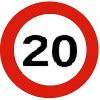
\includegraphics[width=1cm]{./imagenes/2.jpg}  & 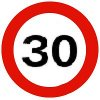
\includegraphics[width=1cm]{./imagenes/3.jpg} & 
\includegraphics[width=1cm]{./imagenes/4.jpg} &  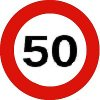
\includegraphics[width=1cm]{./imagenes/5.jpg} &  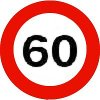
\includegraphics[width=1cm]{./imagenes/6.jpg} \\
      \hline

      Identificador: & 1 & 2 & 3 & 4 & 5 & 6 \\
      \hline
      Figura externa:& 8 & 9 & 9 & 9 & 9 & 9 \\     
      \hline
      Perímetro:& 506.877 & 1025.25 & 1565.18 & 1971.43 & 2510.69 & 2979.51 \\
      \hline 
      Área: & 8384.5 & 12774.5 & 17323.5 & 21771 & 26734 & 30611.5 \\ 
      \hline
      Número de vértices: & 39 & 77 & 125 & 156 & 197 & 236 \\ 
      \hline
      Piezas interiores: & 4 & 2 & 2 & 2 & 2 & 2 \\
      \hline
    \end{tabular}
  \end{center}
  \caption{Tabla con los datos extraídos para algunas de las clases (señales) a identificar.}
  \label{table:tabla-modelos}
\end{table}

Por tanto la matriz de modelos obtenida queda de la siguiente manera:\\

\[
 M =
 \begin{pmatrix}
  1 & 2 & 3 & 4 & 5 & 6 & 7 & 8 & \cdots\\
  8 & 9 & 9 & 9 & 9 & 9 & 9 & 9 & \cdots\\     
  506.877 & 1025.25 & 1565.18 & 1971.43 & 2510.69 & 2979.51 & 3406.49 & 3828.48 & \cdots\\
  4001 8384.5 & 12774.5 & 17323.5 & 21771 & 26734 & 30611.5 & 35896.5 & 40857 & \cdots\\ 
  39 & 77 & 125 & 156 & 197 & 236 & 264 & 299 & \cdots\\
  4 & 2 & 2 & 2 & 2 & 2 & 2 & 2 & \cdots\\
 \end{pmatrix}
\]

\subsection{Clasificación}

Para la clasificación se ha empleado un algoritmo denominado \emph{el vecino más cercano} haciendo uso de los datos extraídos del objeto desconocido y de la matriz modelos obtenida durante la etapa de entrenamiento. \\

Para proceder a la extracción de los datos del objeto desconocido se ha realizado los mismos pasos que durante la etapa de entrenamiento solo que aplicándose a una imagen de entrada, en lugar de aplicarse con las imágenes reservadas para entrenar el sistema.\\

Una vez obtenido el vector de característica del elemento desconocido, se realiza la llamada al algoritmo del vecino más cercano recibiendo la matriz de modelos previamente obtenida de la etapa de entrenamiento junto con el vector de característica del objeto a identificar. La figura \ref{math:vector-columna} muestra una imagen representativa de un vector característica del que cuya clase de pertenencia es desconocida:\\

\begin{figure}[H]
  \begin{center}
    \[
    Vdesconocido =
    \begin{pmatrix}
      8\\     
      502.237 \\
      4022 \\ 
      34 \\
      4 
      \nocite{}
    \end{pmatrix}
    \]
  \end{center}
  \caption{Vector de características de un elemento desconocido.}
  \label{math:vector-columna}
\end{figure}

Como podemos apreciar, el objeto desconocido (del que no se conoce su clase) es representado por una matriz columna. A continuación se calcula la distancia euclídea entre cada uno de los vectores columnas integrantes de la matriz modelos y el vector desconocido, seleccionándose el ejemplo más cercano. El nuevo ejemplo es clasificado con la clase que pertenece el vector seleccionado dentro de la matriz modelos.\\

Este método supone que el vecino más cercano nos dé la mejor clasificación y esto se hace utilizando todos los atributos; el problema de dicha suposición es que es posible que se tengan muchos atributos irrelevantes que dominen sobre la clasificación: dos atributos relevantes perderían peso entre otros irrelevantes.\\

A continuación se muestra la fórmula para el cálculo de la distancia euclídea, definida como la raíz cuadrada de las sumas de las diferencias de las componentes al cuadrado:\\

\begin{figure}[H]
  \begin{center}
    \[
    d(x_{i},y_{j}) = \sqrt{\sum_{r=1}^p (x_{ir}-x_{jr})^2}
    \nocite{}
    \]
  \end{center}
  \label{eq:dist-euclid}
  \caption{Fórmula para el cálculo de la distancia euclídea, definida como la raíz cuadrada de las sumas de las diferencias de cada una de las componentes del vector al cuadrado.}
\end{figure}

A continuación se muestra el código realizado para la clasificación utilizando el algoritmo del vecino más cercano:\\

\underline{Aplicación del vecino más cercano}\\
\begin{Verbatim}[commandchars=\\\{\}]
\PY{k+kt}{int} \PY{n}{Clasificador}\PY{p}{(}\PY{n}{CvMat} \PY{n}{DatosEntrenamiento}\PY{p}{,} \PY{n}{CvMat} \PY{n}{DatosCandidato}\PY{p}{)}\PY{p}{\PYZob{}}

  \PY{c+c1}{// Aplicación del algoritmo KNN.}
  
  \PY{k}{const} \PY{k+kt}{int} \PY{n}{K} \PY{o}{=} \PY{l+m+mi}{1}\PY{p}{;} \PY{c+c1}{// Se fija valor de K. (K=1, vecino más cercano).}
  \PY{k+kt}{int} \PY{n}{solucion}\PY{p}{;}    \PY{c+c1}{// Solución}
  
  \PY{c+c1}{// Se crea e inicializa el vector de clases, cada elemento columna de }
  \PY{c+c1}{// DatosEntrenamiento es una clase}
  
  \PY{k+kt}{int} \PY{n}{clases}\PY{p}{[}\PY{n}{elementos}\PY{p}{]}\PY{p}{;}	
  \PY{n}{CvMat}  \PY{n}{Clases} \PY{o}{=} \PY{n}{cvMat}\PY{p}{(}\PY{n}{elementos}\PY{p}{,}\PY{l+m+mi}{1}\PY{p}{,} \PY{n}{CV\PYZus{}32FC1}\PY{p}{,}\PY{n}{clases}\PY{p}{)}\PY{p}{;}
  
  \PY{k}{for} \PY{p}{(}\PY{k+kt}{int} \PY{n}{a}\PY{o}{=}\PY{l+m+mi}{0}\PY{p}{;}\PY{n}{a}\PY{o}{<}\PY{n}{DatosEntrenamiento}\PY{p}{.}\PY{n}{rows}\PY{p}{;}\PY{n}{a}\PY{o}{+}\PY{o}{+}\PY{p}{)}\PY{p}{\PYZob{}}
    \PY{k}{for} \PY{p}{(}\PY{k+kt}{int} \PY{n}{b}\PY{o}{=}\PY{l+m+mi}{0}\PY{p}{;}\PY{n}{b}\PY{o}{<}\PY{n}{Clases}\PY{p}{.}\PY{n}{cols}\PY{p}{;}\PY{n}{b}\PY{o}{+}\PY{o}{+}\PY{p}{)}\PY{p}{\PYZob{}}
      \PY{c+c1}{// Se añaden los identificadores.}
      \PY{n}{cvSetReal2D}\PY{p}{(}\PY{o}{&}\PY{n}{Clases}\PY{p}{,}\PY{n}{a}\PY{p}{,}\PY{n}{b}\PY{p}{,}\PY{n}{a}\PY{o}{+}\PY{l+m+mi}{1}\PY{p}{)}\PY{p}{;}
    \PY{p}{\PYZcb{}}
  \PY{p}{\PYZcb{}}
  
  \PY{c+c1}{// Se crea el clasificador.}
  \PY{n}{CvKNearest} \PY{n}{knn}\PY{p}{(} \PY{o}{&}\PY{n}{DatosEntrenamiento}\PY{p}{,} \PY{o}{&}\PY{n}{Clases}\PY{p}{,} \PY{l+m+mi}{0}\PY{p}{,} \PY{n+nb}{false}\PY{p}{,} \PY{n}{K} \PY{p}{)}\PY{p}{;}
  \PY{n}{CvMat}\PY{o}{*} \PY{n}{nearests} \PY{o}{=} \PY{n}{cvCreateMat}\PY{p}{(} \PY{l+m+mi}{1}\PY{p}{,} \PY{n}{K}\PY{p}{,} \PY{n}{CV\PYZus{}32FC1}\PY{p}{)}\PY{p}{;}
  
  \PY{c+c1}{// Se estima el vecino más cercano.}
  \PY{n}{solucion} \PY{o}{=} \PY{n}{knn}\PY{p}{.}\PY{n}{find\PYZus{}nearest}\PY{p}{(}\PY{o}{&}\PY{n}{DatosCandidato}\PY{p}{,}\PY{n}{K}\PY{p}{,}\PY{l+m+mi}{0}\PY{p}{,}\PY{l+m+mi}{0}\PY{p}{,}\PY{n}{nearests}\PY{p}{,}\PY{l+m+mi}{0}\PY{p}{)}\PY{p}{;}
   
  \PY{c+c1}{// Se devuelve el resultado.}
  \PY{k}{return}  \PY{n}{solucion}\PY{p}{;}
\PY{p}{\PYZcb{}}
\end{Verbatim}



\subsection{Problemas detectados}

Los problemas que han llevado a cabo el rechazo de este segundo prototipo han sido los siguientes:

\begin{itemize}

\item Los datos obtenidos durante la extracción de características tales como área, perímetro, número de vértices, número de objetos interiores de la señal, entre otros, no resultaban determinantes y excluyentes a la hora de realizar la clasificación proporcionando un alto número de errores cuando el objetivo es elaborar un sistema lo más fiable y eficiente posible.

\item Como punto positivo, se ha comprobado que el algoritmo de los k-vecinos presenta un funcionamiento más adecuado a las características exigibles del proyecto trabajando con los datos de entrada adecuados ya que proporciona una buena relación entre tiempo computacional y efectividad. Por otro lado, el algoritmo presenta la posibilidad de identificación de más de una clase ya que como entrada es capaz de recibir datos de distintas clases a identificar como no ocurría con la comparación de plantillas . Por estas razones se ha considerado adecuado continuar el desarrollo del siguiente prototipo haciendo uso del algoritmo K-vecinos más cercanos cambiando los datos de entrada por otro conjunto de datos que hagan mejorar su funcionamiento.

\end{itemize}

\section{Tercer y último prototipo}

Dado que el prototipo anterior presentaba una baja relación de aciertos, y observando la idoneidad de continuar con el algoritmo del k-vecinos más cercano con valores de K = 1. Se ha optado por continuar con la misma técnica de clasificación cambiando los datos integrantes de la matriz de modelos por unos más representativos.

\subsection{Extracción de características}

Para la extracción de las características necesarias para la creación de la matriz de modelos por parte del algoritmo de entrenamiento han sido necesarias una serie de etapas que se describen en las sucesivas secciones.

\subsubsection{Segmentación por color}

Como etapa inicial, se ha seguido con la metodología empleada en el segundo prototipo utilizando, del igual modo, una segmentación por color aplicando el modelo de color HSV. La única salvedad radica en que en esta ocasión se han añadido los valores necesarios para filtrar las tonalidades azules. En la sección \ref{sec:color-HSV}, referente al segundo prototipo, se describe al detalle la metodología seguida.

\subsubsection{Obtención de datos representativos}

En esta ocasión se ha procedido extraer de forma separada los elementos interiores de una señal de tráfico, para ello a cada objeto identificado tras la selección de color se le aplica un relleno y se extrae mediante máscaras el objeto de la imagen original siguiendo la misma metodología que en el primer prototipo. Ver sección \ref{sec:extraccion-objetos} para consultar el proceso detalladamente.\\

Posteriormente, la imagen obtenida con el objeto candidato es pasada a escala de grises y se identificaban los contornos. Cada uno de los contornos detectados se corresponden con un elemento interno de la posible señal de tráfico. Los contornos son dibujados rellenando sus huecos vacíos con el fin de eliminar los contornos interiores.\\

Cada elemento es a su vez extraído en una nueva imagen donde es redimensionado a un tamaño fijado y dispuesto en un vector columna, dicho vector columna es utilizado para ser agregado a la matriz modelos. La figura \ref{fig:pasos-prototipo3} muestra una representación del proceso seguido. \\


\begin{figure}[H]
  \begin{center}
      \begin{tabular}{ccccc p{3cm}p{3cm}p{3cm}p{1cm}}
        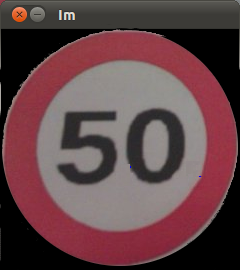
\includegraphics[width=3cm]{./imagenes/mascara/mascara3.png} &  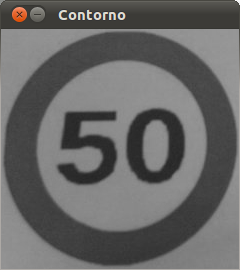
\includegraphics[width=3cm]{./imagenes/prototipo3/Contornogris.png} &  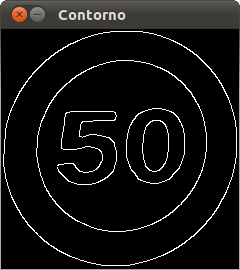
\includegraphics[width=3cm]{./imagenes/prototipo3/contorno.png} &  
\includegraphics[width=0.95cm]{./imagenes/prototipo3/elementos2.png} \\
        {(\emph{a})} & {(\emph{b})} & {(\emph{c})} & {(\emph{d})} \\
      \end{tabular}
    \caption{Proceso seguido para la extracción de los objetos interiores de una señal.}
    \label{fig:pasos-prototipo3}
  \end{center}
\end{figure}

En la imagen (\emph{d}) de la figura \ref{fig:pasos-prototipo3} se visualiza el elemento 0 y el 5 por separado. Ambas matrices representativas de las imágenes, junto con las del resto de elementos a identificar, son dispuestas en vectores columnas y agregadas a la matriz de modelos junto con su identificador, se ha empleado como identificador un carácter numérico para el caso de los números, caracteres alfabéticos para las letras implicadas como las existentes en la señal de Stop y otros caracteres para el resto de elementos como las flechas indicadoras de dirección. Ver figuras \ref{fig:representacion-cinco} y \ref{fig:representacion-columna-cinco}.\\

\begin{figure}[H]
  \begin{center}
    \[
    V_1 =
    \begin{pmatrix}
      1 & 1 & 1 & 1 & 1 & 1 & 1 & 1\\
      1 & 1 & 1 & 1 & 1 & 1 & 1 & 1\\
      1 & 1 & 0 & 0 & 0 & 0 & 0 & 0\\ 
      1 & 1 & 0 & 0 & 0 & 0 & 0 & 0\\ 
      1 & 1 & 1 & 1 & 1 & 1 & 1 & 1\\    
      1 & 1 & 1 & 1 & 1 & 1 & 1 & 1\\
      0 & 0 & 0 & 0 & 0 & 0 & 1 & 1\\ 
      0 & 0 & 0 & 0 & 0 & 0 & 1 & 1\\
      1 & 1 & 1 & 1 & 1 & 1 & 1 & 1\\
      1 & 1 & 1 & 1 & 1 & 1 & 1 & 1\\
    \end{pmatrix}
    \]
    \caption{Representación del número cinco en una matriz.}
    \label{fig:representacion-cinco}
  \end{center}
\end{figure}

\begin{figure}[H]
  \begin{center}
    \[
    V_2 =
    \begin{pmatrix}
      5 \\ 1 \\ 1 \\ 1 \\ 1 \\ 1 \\ 1 \\ 1 \\ 1\\ \vdots\\ 1 \\ 1 \\ 1
    \end{pmatrix}
    \]
    \caption{Resultado de la transformación de la matriz $V_1$ en vector columna añadiendo las diferentes columnas de $V_1$ sucesivamente una bajo la otra en $V_2$. El vector resultante posee en la primera posición el identificador de la clase, en el caso mostrado el carácter ``5''.}
    \label{fig:representacion-columna-cinco}
  \end{center}
\end{figure}

\subsection{Clasificación}

Para proceder con la clasificación, previamente la matriz modelos es cargada de un fichero donde se encuentra almacenada.\\

Antes de realizar la clasificación hay que procesar la imagen de entrada del mismo modo que se ha realizado durante la etapa de entrenamiento. Cada elemento existente dentro de una figura circular roja es extraído y dispuesto en un vector columna para ser clasificado mediante el algoritmo del vecino más cercano. Supongamos la señal de 50km/h. Sus elementos interiores son el carácter ``5'' y el carácter ``0''. Por tanto, si se aplica el algoritmo del vecino más cercano nos producirá como salida en la primera llamada un ``5'' y en la segunda un ``0''. Dado que ambos elementos se encuentran dentro de una circunferencia de color rojo, se determina que el objeto procesado se trata de la señal de 50km/h. Ver figura \ref{fig:salida-protot3}. \\

\begin{figure}[H]
  \begin{center}
        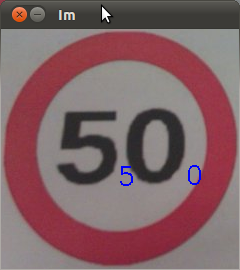
\includegraphics[width=3cm]{./imagenes/prototipo3/salida3.png}
  \end{center}
    \caption{Identificación de los elementos interiores de la señal, el valor ``5'' y el valor ``0'', determinándose el objeto como una señal de 50 km/h.}
    \label{fig:salida-protot3}
\end{figure}

El algoritmo de clasificación empleado ha sido el mismo que el utilizado en el prototipo anterior con la salvedad de que en esta ocasión se rechazan aquellos valores de salida cuya distancia supera un determinado umbral. Con esta modificación los elementos serán clasificados cuando su grado de parentesco es elevado y no con la clase con la que más se le parece aunque sea un objeto totalmente diferente.\\

A continuación se muestra el código modificado:\\

\underline{Algoritmo del vecino más cercano modificado para la obtención de las distancias}\\

\begin{Verbatim}[commandchars=\\\{\}]
\PY{k+kt}{int} \PY{n}{Clasificador}\PY{p}{(}\PY{n}{CvMat} \PY{n}{DatosEntrenamiento}\PY{p}{,} \PY{n}{CvMat} \PY{n}{DatosCandidato}\PY{p}{)}\PY{p}{\PYZob{}}

  \PY{c+c1}{// Aplicación del algoritmo KNN.}
  
  \PY{k}{const} \PY{k+kt}{int} \PY{n}{K} \PY{o}{=} \PY{l+m+mi}{1}\PY{p}{;} \PY{c+c1}{// Se fija valor de K. (K=1, vecino más cercano).}
  \PY{k+kt}{int} \PY{n}{solucion}\PY{p}{;}    \PY{c+c1}{// Solución}
  \PY{k+kt}{int} \PY{n}{umbral\PYZus{}minimo} \PY{o}{=} \PY{l+m+mi}{10000}\PY{p}{;} \PY{c+c1}{// Grado de semejanza exigido.}

  \PY{c+c1}{// Vector donde se almacenarán las distancias.}
  \PY{n}{CvMat}\PY{o}{*} \PY{n}{distancias} \PY{o}{=} \PY{n}{cvCreateMat}\PY{p}{(}\PY{l+m+mi}{1}\PY{p}{,}\PY{n}{K}\PY{p}{,}\PY{n}{CV\PYZus{}32FC1}\PY{p}{)}\PY{p}{;}
 
  
  \PY{c+c1}{// Se crea e inicializa el vector de clases, cada elemento columna de }
  \PY{c+c1}{// DatosEntrenamiento es una clase.}
 
  \PY{k+kt}{int} \PY{n}{clases}\PY{p}{[}\PY{n}{elementos}\PY{p}{]}\PY{p}{;}	
  \PY{n}{CvMat}  \PY{n}{Clases} \PY{o}{=} \PY{n}{cvMat}\PY{p}{(}\PY{n}{elementos}\PY{p}{,}\PY{l+m+mi}{1}\PY{p}{,} \PY{n}{CV\PYZus{}32FC1}\PY{p}{,}\PY{n}{clases}\PY{p}{)}\PY{p}{;}
  
  \PY{k}{for} \PY{p}{(}\PY{k+kt}{int} \PY{n}{a}\PY{o}{=}\PY{l+m+mi}{0}\PY{p}{;}\PY{n}{a}\PY{o}{<}\PY{n}{DatosEntrenamiento}\PY{p}{.}\PY{n}{rows}\PY{p}{;}\PY{n}{a}\PY{o}{+}\PY{o}{+}\PY{p}{)}\PY{p}{\PYZob{}}
    \PY{k}{for} \PY{p}{(}\PY{k+kt}{int} \PY{n}{b}\PY{o}{=}\PY{l+m+mi}{0}\PY{p}{;}\PY{n}{b}\PY{o}{<}\PY{n}{Clases}\PY{p}{.}\PY{n}{cols}\PY{p}{;}\PY{n}{b}\PY{o}{+}\PY{o}{+}\PY{p}{)}\PY{p}{\PYZob{}}
      \PY{c+c1}{// Se añaden los identificadores.}
      \PY{n}{cvSetReal2D}\PY{p}{(}\PY{o}{&}\PY{n}{Clases}\PY{p}{,}\PY{n}{a}\PY{p}{,}\PY{n}{b}\PY{p}{,}\PY{n}{a}\PY{o}{+}\PY{l+m+mi}{1}\PY{p}{)}\PY{p}{;}
    \PY{p}{\PYZcb{}}
  \PY{p}{\PYZcb{}}
  
  \PY{c+c1}{// Se crea el clasificador.}
  \PY{n}{CvKNearest} \PY{n}{knn}\PY{p}{(} \PY{o}{&}\PY{n}{DatosEntrenamiento}\PY{p}{,} \PY{o}{&}\PY{n}{Clases}\PY{p}{,} \PY{l+m+mi}{0}\PY{p}{,} \PY{n+nb}{false}\PY{p}{,} \PY{n}{K} \PY{p}{)}\PY{p}{;}
  \PY{n}{CvMat}\PY{o}{*} \PY{n}{nearests} \PY{o}{=} \PY{n}{cvCreateMat}\PY{p}{(} \PY{l+m+mi}{1}\PY{p}{,} \PY{n}{K}\PY{p}{,} \PY{n}{CV\PYZus{}32FC1}\PY{p}{)}\PY{p}{;}
  
  \PY{c+c1}{// Se estima el vecino más cercano.}
  \PY{n}{solucion} \PY{o}{=} \PY{n}{knn}\PY{p}{.}\PY{n}{find\PYZus{}nearest}\PY{p}{(}\PY{n}{elemento\PYZus{}analisis}\PY{p}{,}\PY{n}{K}\PY{p}{,}\PY{l+m+mi}{0}\PY{p}{,}\PY{l+m+mi}{0}\PY{p}{,}\PY{n}{nearests}\PY{p}{,}\PY{n}{distancias}\PY{p}{)}\PY{p}{;}
   
  \PY{c+c1}{//Si hay bastante semejanza, aceptamos como válido. }
  \PY{k}{if} \PY{p}{(}\PY{n}{cvGetReal2D}\PY{p}{(}\PY{n}{distancias}\PY{p}{,}\PY{l+m+mi}{0}\PY{p}{,}\PY{l+m+mi}{0}\PY{p}{)} \PY{o}{<} \PY{n}{umbral\PYZus{}minimo}\PY{p}{)}\PY{p}{\PYZob{}} 
	\PY{k}{return} \PY{n}{solucion}\PY{p}{;}
  \PY{p}{\PYZcb{}}
  \PY{c+c1}{// Si no se devuelve cero.}
  \PY{k}{return}  \PY{l+m+mi}{0}\PY{p}{;}
\PY{p}{\PYZcb{}}
\end{Verbatim}



